%%%%%%%%%%%%%%%%%%%%%%%%%%%%%%%%%%%%%%%%%%%%%%%%%%%%%%%%%%%%%%%%%%%%%%%%%%%%%
%% obtained from https://canvas.uva.nl/courses/6063/files/folder/Templates %%
%%%%%%%%%%%%%%%%%%%%%%%%%%%%%%%%%%%%%%%%%%%%%%%%%%%%%%%%%%%%%%%%%%%%%%%%%%%%%
\documentclass{uvamath}
\usepackage[english]{babel}


\usepackage{graphicx}
\graphicspath{{assets/}}
\usepackage{graphbox}
\usepackage{amssymb}
\usepackage{amsmath}
\usepackage{amsthm}
\usepackage{stmaryrd}
\usepackage[pdfborder={0 0 0}]{hyperref}

\usepackage{csquotes,xpatch} % Recommended by biblatex
\usepackage[
    style=numeric]{biblatex}
\addbibresource{zotero.bib}
\addbibresource{manual.bib}

\newcommand{\N}{\mathbb{N}}


\title{Local Flags: Bounding the Strong Chromatic Index} % Title of your thesis
\author[eoin.davey@student.uva.nl, 14246287]{Eoin Davey} %Your name, email and student number

\documentTitle{Master Thesis}
\program{MSc Mathematics} % MSc Mathematics / MSc Mathematical Physics / Stochastics and Financial Mathematics

\supervisorsTitle{Dr. J.R. Kang} %This is the list of supervisors for the title page, seperate with \newline

\supervisors{Dr. J.R. Kang} %This is the list of supervisors for the second page, seperate with comma

\secondexaminer{Dr. K. Guo} %This is the name of the second examiner, for the second page
\date{June 28, 2024} %This is the examination date, i.e. the date of your thesis presentation

\newtheorem{theorem}{Theorem}[chapter]
\newtheorem{lemma}[theorem]{Lemma}
\newtheorem{corollary}{Corollary}[theorem]
\newtheorem*{knowntheorem}{Theorem}
\newtheorem{conjecture}{Conjecture}
\newtheorem*{knownconjecture}{Conjecture}
\newtheorem*{note}{Note}
\newtheorem{definition}{Definition}[chapter]
\newtheorem*{example}{Example}

\begin{document}
\maketitle

\begin{abstract}
Scientific abstract (5-10 lines)
\end{abstract}

\tableofcontents

\chapter*{Introduction}
\addcontentsline{toc}{chapter}{Introduction}

Consider a simple\footnote{An undirected graph with no self loops and at most 1 edge between any two
vertices.} graph $G$. How many colours do you need to colour the edges such that no two edges which touch
have the same colour? What if no two edges which touch some common edge can have the same colour?
Erd\H{o}s and Nešetřil conjectured that you only need $1.25\Delta(G)^2$ colours where $\Delta(G)$ denotes the maximum degree of $G$, but
the current best proof only shows an upper bound of $1.772\Delta(G)^2$ colours (for large enough $\Delta(G)$). In this thesis
we show how we can lower this to $1.73\Delta(G)^2$ by introducing a novel framework
which is a modification of Razborov's flag algebras. We also apply this new framework
to some other problems including a bounded-degree variant of the
Erd\H{o}s's pentagon conjecture.

\section*{Strong Edge Colouring}
\addcontentsline{toc}{section}{Strong Edge Colouring}
\label{sec:intro_strong_edge_coloring}

An edge colouring of a simple graph $G$ is an assignment $c\colon E(G) \to [k]$
for some $k\in\N$. Such a colouring is \textit{proper} if no two incident\footnote{Have a vertex in common}
edges have the same colour.
An edge colouring is \textit{strong} if no two edges which share a common incident edge have
the same colour. Put differently, proper edge colouring requires edges at distance 1 to have distinct
colours and strong edge colouring extends this to distance 2.
In figure \ref{fig:proper-strong-example} we see an example of a non-proper edge colouring,
a proper (but not strong) edge colouring and a strong edge colouring of $C_5$, the cycle on $5$ vertices.

\begin{figure}[h]
    \centering
    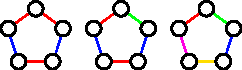
\includegraphics[scale=1.5]{proper-strong-example}
    \caption{Non-Proper, Proper \& Strong Edge Colourings}
    \label{fig:proper-strong-example}
\end{figure}

The \textit{chromatic index} of $G$, denoted $\chi'(G)$, is the minimum $k$ such that a proper edge
colouring of $G$ with $k$ colours exists. The \textit{strong chromatic index} $\chi'_s(G)$
is the corresponding minimum number of colours required for a strong edge colouring.

Vizing's theorem is a well known result which tells us $\chi'(G)$ almost exactly in terms of
the max degree of the graph $\Delta(G)$:
\begin{knowntheorem}[Vizing, 1965 \cite{Vizing_1965}]
    $\Delta(G) \leq \chi'(G) \leq \Delta(G) + 1$.
\end{knowntheorem}
Erd\H{o}s and Nešetřil conjectured in 1985 that
the strong chromatic index can also be bounded precisely by a function of the max degree:
\begin{knownconjecture}[Erd\H{o}s and Nešetřil, see~\cite{faudreeInducedMatchingsBipartite1989}]
    \label{conj:intro_erdos_nesetril}
    $\chi'_s(G) \leq \frac{5}{4}\Delta(G)^2$.
\end{knownconjecture}
The simple construction of a $C_5$, with each vertex substituted with an independent set of size $\Delta(G)/2$, shows that this conjecture would be best possible if true.

A greedy argument shows a bound of $\chi'(G) \leq 2\Delta(G)^2 + o(\Delta(G)^2)$ but it wasn't until
1997 that Molloy and Reed broke the factor $2$ barrier \cite{molloyBoundStrongChromatic1997}.
A series of papers have since made progress on lowering this bound closer to $\frac{5}{4}\Delta(G)^2$.

For $\Delta(G)$ large enough we have the following theorems:
\begin{enumerate}
  \item \textit{Molloy \& Reed, 1997} \cite{molloyBoundStrongChromatic1997}:
        $\chi'_s(G) \leq 1.998\Delta(G)^2$.
  \item \textit{Bruhn \& Joos, 2015} \cite{bruhnStrongerBoundStrong2018}:
        $\chi'_s(G) \leq 1.93\Delta(G)^2$.
  \item \textit{Bonamy, Perrett \& Postle, 2018} \cite{bonamyColouringGraphsSparse2018}:
        $\chi'_s(G) \leq 1.835\Delta(G)^2$.
  \item \textit{Hurley, de Joannis de Verclos \& Kang, 2022} \cite{hurleyImprovedProcedureColouring2022}:
        $\chi'_s(G) \leq 1.772\Delta(G)^2$.
\end{enumerate}

In this thesis we will show how we brought this bound down even further to $1.73\Delta(G)^2$:
\begin{knowntheorem}
    For $\Delta(G)$ large enough we have
    $\chi'_s(G) \leq 1.73\Delta(G)^2$.
\end{knowntheorem}

The 1997 paper by Molloy \& Reed introduced a method for strong edge colouring we call the
\textit{2-step strategy}:
\begin{enumerate}
    \item Find an upper bound for the \textit{strong neighbourhood density} of $G$ in terms of
        $\Delta(G)$.
    \item Use a probabilistic colouring method which uses the previous bound to achieve a colouring
        with a low number of colours.
\end{enumerate}
This method has been modified by the papers which followed the Molloy \& Reed paper but this
strategy has remained the core idea. We will look at this strategy in more detail (including
defining strong neighbourhood density) in chapter \ref{chap:strong_edge_colouring}.
For this thesis we focus on the Step~1, using the Step~2 as a black box. We will
find a new, lower, upper-bound on the strong neighbourhood density and hence achieve our
new strong chromatic index bound.

\section*{Flag Algebras}
\addcontentsline{toc}{section}{Flag Algebras}

Step~1 of the 2-step strategy
asks us to find an upper bound on the strong neighbourhood density. The strong neighbourhood
density belongs to a broad family of density functions which ask: ``How many copies of some
structure $F$ do we find in some larger structure $G$, expressed as a real number $\in [0,1]$''?
These density functions usually count the number of copies of $F$ in $G$, then normalise by the
maximum possible number of such copies.
For example, the density of edges in some graph $G$ is $|E(G)|/\binom{|G|}{2}$.

Bounding densities
is a common problem in combinatorics and in 2007 Razborov \cite{razborovFlagAlgebras2007}
introduced a framework called \textit{flag algebras}
which can be used to prove asymptotic results about densities in various combinatorial settings.
These flag algebras are defined very generally in terms of finite model theory in \cite{razborovFlagAlgebras2007} but we focus on their use with respect to simple graphs.

We give a brief flavour of flag algebras here but defer a full exposition until
chapter \ref{chap:classic_flags}.

\subsection*{A motivating example}
\label{sec:motivating_example}

As a reminder, for a graph $G$ and subset of vertices $U\subseteq V(G)$ the \textit{induced subgraph}
$G[U]$ is the subgraph of $G$ consisting of the vertices in $U$ and all edges between them.
We can then define the \textit{induced count} of $F$ in $G$, denoted $c(F; G)$, as
the number of subsets $U\subseteq V(G)$ such that $G[U] \cong F$. Then we define the
\textit{induced density} as $p(F; G) := c(F; G) / \binom{|G|}{|F|}$.

\begin{note*}
    $p(F; G)$ is precisely the same as the probability that $G[U] \cong F$ if
    $U \subseteq V(G)$ is a uniformly random subset of size $|F|$. This is often
    the more useful way to interpret $p(F;G)$.
\end{note*}

What are some simple algebraic relationships between small subgraphs?
Consider picking 2 vertices at random: then either they form an edge or they don't.
Hence $p(\edge; G) + p(\nonedge; G) = 1$. In general, the sum of densities of all
flags of some size $k$ is always 1. e.g. 
\[ 
    p(\triangleflag; G) + p(\triangletwoedge; G) + p(\triangleoneedge; G)
    + p(\triangleempty; G) = 1.
\]
Now we note that we can sample 2 vertices uniformly at random by
first sampling a triple of vertices at random, and then sampling 2 of those 3 uniformly randomly
again. This lets us derive us the following relation:
\[
    p(\edge; G) = 
    p(\triangleflag; G)
    + \frac{2}{3}p(\triangletwoedge; G)
    + \frac{1}{3}p(\triangleoneedge; G)
    + 0\cdot p(\triangleempty; G)
\]
A similar thought experiment relating sampling two pairs uniformly at random to sampling 4
vertices and then splitting the 4 randomly into two halves tells us:
\[
    p(\edge; G)^2 \sim p(\kfour; G) + \frac{2}{3}\left(p(\kfourmone; G) + p(\cfour; G)\right)
        + \frac{1}{3}\left(p(\kfourmtwo; G) + p(\kfourbucket; G) + p(\kfourtwopair; G)\right)
\]

Simplifying our notation then we might arrive at a hypothetical symbolic algebra which has relations
like:
\begin{gather*}
    \edge + \nonedge = 1\\
    \triangleflag
    + \triangletwoedge
    + \triangleoneedge
    + \triangleempty = 1\\
    \edge =
    \triangleflag
    + \frac{2}{3}\triangletwoedge
    + \frac{1}{3}\triangleoneedge\\
    \edge^2 =
    \kfour + \frac{2}{3}(\kfourmone + \cfour)
        + \frac{1}{3}(\kfourmtwo + \kfourbucket + \kfourtwopair).
\end{gather*}

We call these graph symbols \textit{flags}.
We can then prove results with simple symbolic manipulation: In a triangle-free graph
we would have $\triangleflag = 0$, hence
\[
    \edge = \frac{2}{3}\triangletwoedge + \frac{1}{3}\triangleoneedge \leq
    \frac{2}{3}(\triangletwoedge + \triangleoneedge)
    \leq \frac{2}{3}(\triangleflag + \triangletwoedge + \triangleoneedge + \triangleempty)
    \leq \frac{2}{3}
\]
as flags are non-negative. This (given all the formal definitions and proofs we've deferred)
is a formal proof
that $p(\edge; G) \leq \frac{2}{3}$ for any triangle-free graph. The best possible result
says that $p(\edge; G) \leq \frac{1}{2}$ and is known as
\textit{Mantel's theorem} \cite{Mantel_1910}. This is
also easily proved with flag algebras which is seen in chapter \ref{chap:classic_flags}.

\subsection*{Computer Search}

One of the most (if not \textit{the most}) important aspects of flag algebras is that
they lend themselves very well to computer search methods.
The flag algebras allow us to prove results using only simple symbol manipulation in a very
tractable way.

In practice we use the \textit{semidefinite method} to optimise some objective function
over the algebra, and due to duality this gives us a rigorous proof of an upper bound on our
function.
We will see in section \ref{sec:semidefinite_method} how we construct the semidefinite program,
and how we can interpret the dual solutions in a more human understandable way.

\section*{Local Flags}
\addcontentsline{toc}{section}{Local Flags}

One might be tempted to try to apply these flag algebras directly to our strong neighbourhood
density problem, but in practice this problem doesn't fit well into the flag algebra model.
In particular, Razborov's flag algebras are constructed to work well with density functions
like the induced density function $p(F; G) = c(F; G)/\binom{|G|}{|F|}$ which have a
denominator which is $\Theta(|G|^{|F|})$. This is convenient if we are trying to prove
a bound on some function which is polynomial in $|G|$
(e.g. Mantel's theorem says the number of edges is $\leq \frac{1}{4}|G|^2$). But what if
we want to prove a bound on a function which is polynomial in some other function
of $G$? e.g. The \hyperref[conj:intro_erdos_nesetril]{Erd\H{o}s-Nešetřil Conjecture}
wants to bound $\chi'_s(G)$ with a polynomial in $\Delta(G).$ This does not lend itself
to the same methods.

Instead, we can define a new ``density'' function which instead normalises our induced
count by a different denominator: one which captures the graph parameter we want to measure
our count ``relative to''. In particular, in chapter \ref{chap:local_flags} we introduce a
new \textit{local density function} and a concept we call a \textit{local flag}.
We show that, under certain conditions, these local flags also form a nice algebra
with which we can apply the semidefinite method to prove bounds.

\section*{Contributions and Results}
\addcontentsline{toc}{section}{Contributions and Results}

The work in this thesis was completed with valuable contributions from Rémi de Joannis de Verclos,
Eoin Hurley, Jan Volec and my supervisor Ross Kang.

The concept for this new framework was originally explored\footnote{In unpublished notes.} by Rémi de Joannis de Verclos in
2020, in collaboration with Eoin Hurley and Ross Kang.
He conjectured the structure of the framework, then adapted flag algebra
software\footnote{\url{https://crates.io/crates/flag-algebra}}
to test if this framework could in principle improve on existing results.
This experiment showed that if the framework could be realised formally then it could improve the
best known bound on the strong chromatic index.

The conjecture which motivates chapter \ref{chap:pentagon_conjecture}, the
proof of lemma \ref{lemma:pentagon_1_8_tight} and the definition of $Q(G,v)$ in
section \ref{sec:pentagon_stronger} were conceived in discussion with Eoin Hurley.

\hfill

Using our new framework which is introduced in chapter \ref{chap:local_flags}
we have made progress on several open problems:
\begin{itemize}
    \item In chapter \ref{chap:pentagon_conjecture} we show a ``warmup'' application of the new
        framework: We state a new conjecture which is a bounded-degree version of the famous
        Erd\H{o}s pentagon conjecture \cite{erdos_pentagon_1984}.
        We then show how a relatively straightforward application of the local flags method makes non-trivial
        progress towards proving the conjecture, and show that a slightly more complex application
        then gets even closer to the full result.
        This problem came about naturally as the original pentagon conjecture was originally resolved using
        the classic flag algebras (\cite{hatamiNumberPentagonsTrianglefree2013},
        \cite{grzesikMaximumNumberFivecycles2012}).
    \item In chapter \ref{chap:strong_edge_colouring} we apply this new framework to make progress on the
        \hyperref[conj:intro_erdos_nesetril]{Erd\H{o}s-Nešetřil Conjecture}, achieving the best-yet
        bound of $\chi'_s(G) \lesssim 1.73\Delta(G)^2$. The approach used here is a modification
        of the approach conjectured by de Joannis de Verclos.
    \item At the end of chapter \ref{chap:strong_edge_colouring} we alter the method to make
        the first targeted progress on the special bipartite version of this conjecture, showing that
        if $G$ is bipartite then we have the bound $\chi'_s(G) \lesssim 1.6254\Delta(G)^2$. We also
        investigate the asymmetric version of this bipartite case and make an interesting discovery
        where the chromatic bound is constant across all degrees of asymmetry.
\end{itemize}

At the end of the document you will find 3 appendices which might be of interest.
\begin{itemize}
    \item Appendix \ref{app:notation} lists some notation as a reference.
    \item Appendix \ref{app:flag_software} gives some practical details on how the SDP
        software was written, and where to find it.
    \item Appendix \ref{app:sdp_verification} gives some light details on how the solutions
        to SDP problems were, or could be, verified.
\end{itemize}


\chapter{Background: Classic Flag Algebras}
\label{chap:classic_flags}

In the first section we will briefly introduce Razborov's flag algebras as they apply to
graphs. If the reader is already familiar with flag algebras this section can be skipped.

In the second section we will discuss how the semidefinite method is applied to flag algebras.
The method we use is slightly different to the method used in other works
(e.g. \cite{silvaFlagAlgebrasFirst2016}) but is more easily adapted to our new framework.

\section{Flag Algebras}

All the following definitions are concepts from \cite{razborovFlagAlgebras2007}, rephrased
to focus only on the simple graph case.
For similar introductions to flag algebras we point the reader to
\textit{Flag Algebras: A First Glance} by Silva, Filho and Sato
\cite{silvaFlagAlgebrasFirst2016} and \textit{A Brief Introduction to Flag Algebra} by Qi
\cite{qiBriefIntroductionFlag}.

In our \hyperref[sec:motivating_example]{example} we only discussed counting how many copies of
some $F$ are in some larger
graph $G$, but in practice we often want to be able to ask how many copies are
there of $F$ in $G$ where we force some part of $F$ to be mapped to a specific part of $G$.
For example, if $F=\edge$ and $G$ is any graph then $c(F; G) = |E(G)|$, but if we pick
some vertex $v\in V(G)$ and ask how many copies of $\edge$ are there in $G$ such that the first
vertex in $\edge$ is mapped to $v$ then we get $c(F; G) = \deg v$. This ability to pin down certain
vertices is what really unlocks the potential of flags.

We will represent this action of fixing some subset of vertices by partial labelling,
and just as in our \hyperref[sec:motivating_example]{motivating example} we will create
a algebra out of some small graphs, in a such a way that symbolic operations capture
algebraic relations between the densities of the underlying graphs.

\subsection{Flags}

The fundamental object of our algebra is the \textit{flag} which is a partially
labelled graph, meaning some of the vertices of the graph have integer labels assigned to
them. The \textit{type} of the flag then is the subgraph induced by the labelled vertices.
In figure \ref{fig:flags-types} we see some example flags and their types. The labelled vertices
are represented visually with a partially filled vertex.

\begin{figure}[h]
    \centering
    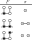
\includegraphics{flags-types-example}
    \caption{Example flags and their types}
    \label{fig:flags-types}
\end{figure}

We give the formal definitions:

\begin{definition}[Type]
    A \textbf{type} $\sigma$ of size $k$ is a graph with vertex set $[k]$. We write
    $|\sigma|$ to denote the size of the underlying graph. We write
    $\emptyset$ to denote the type consisting of the empty graph.
\end{definition}
\begin{definition}[$\sigma$-Embedding]
    Given a type $\sigma$ and a graph $F$, a \textbf{$\sigma$-embedding} is an injective
    function $\theta\colon[|\sigma|]\to V(F)$ which is a graph isomorphism between
    $\sigma$ and $F[\im \theta]$.
\end{definition}
\begin{definition}[$\sigma$-Flag]
    A \textbf{$\sigma$-flag} is a tuple $(F, \theta)$ where $\theta$ is an $\sigma$-embedding
    into $F$.
    If the embedding is implicit (e.g. if $\sigma=\emptyset$) we often drop the
    $\theta$ from the notation.
\end{definition}

\begin{note}
    A type $\sigma$ is implicitly itself a $\sigma$-flag when taken with the
    identity embedding $\id\colon [|\sigma|] \to [|\sigma|]$. We often use this fact
    implicitly.
\end{note}

We then say that two flags are isomorphic if there is a graph isomorphism between the underlying
graphs which preserves the labels.
\begin{definition}[Flag Isomorphism]
    $f\colon V(F) \to V(F')$ is a $\sigma$-flag isomorphism
    from $(F,\theta) \to (F', \theta')$ if it is graph isomorphism $F \to F'$ such that
    $f(\theta(i)) = \theta'(i)\ \forall\ i\in [|\sigma|].$ We can
    write $(F,\theta)\cong (F',\theta')$ if such an $f$ exists.
\end{definition}

Now that we have a definition for flags we can build on our induced density function from
the introduction.

\subsection{Induced Counts and Density}

In the introduction we defined the induced count $c(F; G)$ to be the number of
$U\subseteq V(F)$ such that $G[U] \cong F$. We need to adapt this notion now to handle
labelled vertices which must be preserved by the isomorphism. In particular if $G[U] \cong F$
then $U$ must contain the labelled vertices of $G$.

\begin{definition}[Induced Count]
    Fix two $\sigma$-flags $(F,\theta), (G,\eta).$ We define the induced count of $(F,\theta)$ in
    $(G,\eta)$ written $c((F,\theta); (G,\eta))$
    as the number of subsets $\im(\eta)\subseteq U\subseteq V(G)$ such that
    $(F,\theta) \cong (G[U], \eta)$.\footnote{Where we restrict the codomain of $\eta$ appropriately}
\end{definition}

We can extend this notion of counting how many copies of $F$ there are in $G$ to ask
how many tuples of disjoint copies of $F_1, \dots, F_t$ are there in $G$ (where
disjoint means vertex-disjoint apart from the fixed labelled vertices).

Precisely we define $c(F_1, \dots, F_t; G)$ to be the number of
$U_1, \dots, U_t\subseteq V(G)$ such that $\im\eta = U_i \cap U_j\ \forall\ i, j \in [t]$ where
$i\neq j$ and $(F_i, \theta_i) \cong (G[U_i], \eta)$ for all $i\in [t].$

Note that if $c(F_1, \dots, F_t; G) > 0$ we know that $G$ must be large enough to fit
disjoint copies of $F_1, \dots, F_t$ leading us to the following definition.

\begin{definition}[Fit]
    We say $\sigma$-flags $F_1, \dots, F_t$ \textbf{fit} in $\sigma$-flag $G$ if
    $|G|-|\sigma| \geq \sum_{i=1}^t |F_i|-|\sigma|$.
\end{definition}

\begin{example}
    Consider the type $\sigma=\vertex$, a single vertex. Any $\sigma$-flag $(G,\eta)$ is
    just a graph with a specific distinguished vertex (the unique labelled vertex).

    Consider then the $\sigma$-flag $F=\edgemarked$, an edge with a single labelled vertex.
    For any $G$ with distinguished vertex $v$, $c(\edgemarked; G) = \deg_G(v)$ as explained
    above.

    Similarly, $c(\edgemarked, \edgemarked; G) = \binom{\deg(v)}{2}.$ This is as
    we are counting how many distinct pairs of vertices $(a, b)$ are there in $G$ such that
    $G[\{a, v\}] \cong \edgemarked$ and $G[\{b, v\}] \cong \edgemarked$.
    In other words, how many distinct pairs of vertices are there connected to
    $v$, which is clearly $\binom{\deg(v)}{2}.$
\end{example}

Now we can define the induced density by normalising the induced count by the max
possible number of such non-overlapping $t$-tuples.

\begin{definition}[Induced Density]
    Given $\sigma$-flags $F_1, \dots, F_t$ and $G$ define the \textbf{induced density} of
    $F_1, \dots, F_t$ in $G$ as:
    \[
    p(F_1, \dots, F_t; G)
    := \frac{c(F_1, \dots, F_t; G)}{
    \binom{|G|-|\sigma|}{|F_1|-|\sigma|, \dots,|F_t|-|\sigma|, R}}
    \]
    where we use multinomial coefficient notation with
    $R=(|G|-|\sigma|)-\sum_{i=1}^t |F_i|-|\sigma|$.
\end{definition}

\begin{note}
    Again, as in the \hyperref[sec:motivating_example]{motivating example in the introduction},
    we can interpret $p(F_1, \dots, F_t; G)$ in a precise probabilistic way.
    $p(F_1, \dots, F_t; G)$ is exactly the probability that
    $(F_i, \theta_i) \cong (G[U_i], \eta)\ \forall\ i\in[t]$ where
    $U_1, \dots, U_t \subseteq V(G)$ is a uniformly random $t$-tuple of subsets such that
    $U_i \cap U_j = \im \eta\ \forall i, j \in [t], i \neq j$.
\end{note}

\subsection{Graph Classes}

Often, we want to limit our view to a subset of all possible graphs. For example, we
will want to consider only triangle-free graphs when proving Mantel's theorem (TODO REF).

We pick some class of graphs $\Gcl$. For Razborov's flag algebras we assume that
$\mathcal{G}$ is hereditary, meaning it is closed under taking induced subgraphs. This will change
when we introduce our new local framework.

Then for any type $\sigma$ we write $\Gcl^\sigma$ for the set of all $\sigma$-flags up to
isomorphism. We write $\Gcl^\sigma_n$ for the set of all $\sigma$-flags of size $n$.
We generally assume $\Gcl^\sigma$ is infinite for any type $\sigma\in\mathcal{G}$.
If $\sigma=\emptyset$ we often skip the superscript and just refer to
$\Gcl$ or $\Gcl_n$.

From this point all definitions and results are relative to some fixed graph class
$\mathcal{G}$.

Given some graph class $\mathcal{G}^\sigma$ then we get the very power \textit{chain rule}.
\begin{lemma}[The Chain Rule, Lemma 2.2 \cite{razborovFlagAlgebras2007}]
    \label{lemma:chain_rule}
    If $F_1, \dots, F_t \in \Gcl^\sigma$ are $\sigma$-flags which fit in $G\in\Gcl^\sigma$
    then for all $1 \leq s \leq t$ and every $n$ such that
    $F_1, \dots, F_s$ fit into a $\sigma$ flag of size $n$ and a
    $\sigma$-flag and $F_{s+1}, \dots, F_t$ fit in $G$ we have:
    \[
    p(F_1, \dots, F_t; G) = \sum_{F \in \mathcal{G}^\sigma_n}
    p(F_1, \dots, F_s; F)p(F, F_{s+1}, \dots, F_t; G).
    \]
\end{lemma}

This chain rule is one of the crucial properties that we will lose when we define our
local flags framework.

\subsection{The Algebra}

We've describe now our flags in detail, understanding a partially labelled flag and
the density functions they in some way represent. We would like to then formally
describe a structure on these flags such that relations in the structure describe true
relations about their associated density functions. As a start we want to be able
to describe linear combinations of flags, e.g. $\edge + \nonedge$ should in some
way represent $p(\edge; G) + p(\nonedge; G)$.

Take then the formal real vector space $\R\Gcl^\sigma$ for some fixed type $\sigma$,
this gives us a proper notion of these linear combinations of flags. We can then
linearly extend our density function $p$ to this space in the first argument giving
us a function $p\colon \R\Gcl^\sigma \times \Gcl^\sigma \to \R$ capturing that
$p(\edge + \nonedge; G) = p(\edge; G) + p(\nonedge; G) = 1$ and similar relations.

The chain rule (Lemma \ref{lemma:chain_rule}) tells us then that for any $F, G\in\Gcl^\sigma$
and $n \geq |F|$ we have $p(F; G) = \sum_{H \in \Gcl^\sigma_n}p(F; H)p(H; G)$. In
In particular, $p(F; H)$ is just some real number for each $H$ meaning
$p(F; G) - \sum_{H \in \Gcl^\sigma_n}p(F; H)p(H; G) = 0$ is a linear relation on
density functions which holds for all $F, G$. This tells us that in our algebra
any vector of the form $v = F - \sum_{H \in \Gcl^\sigma_n}p(F; H)H$ has the property
that $p(v; G) = 0$ for all $G\in\Gcl^\sigma$.

We can define the space $\mathcal{K}^\sigma$ as the span of vectors of the form
$F - \sum_{H \in \Gcl^\sigma_n}p(F; H)H$ for $F\in\Gcl^\sigma$, $n\geq |F|$ and
quotient out this relation from $\R\Gcl^\sigma$. Because $p(v; G) = 0$ for all
$v \in\mathcal{K}^\sigma, G \in\mathcal{G}$ our linear extension of $p$ is still well defined
on this space.

\begin{example}
    If $\Gcl$ is the class of triangle free graphs then we know from our
    \hyperref[sec:motivating_example]{motivating example} that
    $p(\edge; G) = \frac{2}{3}p(\triangletwoedge; G) + \frac{1}{3}p(\triangleoneedge; G)$
    for all $G\in\mathcal{G}$. We would like this to translate to a relation like
    $\edge = \frac{2}{3}\triangletwoedge + \frac{1}{3}\triangleoneedge$.

    In the space $\R\Gcl^\emptyset / \mathcal{K}^\emptyset$ both the vectors $\edge$ and
    $\frac{2}{3}\triangleoneedge + \frac{1}{3}\triangleoneedge$ belong to the same
    coset, so they are indeed equal. Hence this space does capture this relationship.
\end{example}

However, linear combinations are not powerful enough. We also want to be able to make
statements about products of densities. Ideally we would be able to define a
product on vectors $f, g \in \R\Gcl^\sigma / \mathcal{K}^\sigma$ such that for any $G\in\Gcl^\sigma$
we have $p(f \cdot g; G) = p(f; G)\cdot p(g; G)$. Unfortunately we don't achieve the
ideal relation, but we do get the result asymptotically which is enough:
$p(f\cdot g; G) = p(f; G) \cdot p(g; G) + o(1)$.

\begin{definition}[$\sigma$ Flag Algebra]
    For fixed type $\sigma$ define the following product $\Gcl^\sigma \times \Gcl^\sigma \to \R\Gcl^\sigma / \mathcal{K}^\sigma$
    on $\sigma$-flags $F, G\in\Gcl^\sigma$.
    \[
        F \cdot G := \sum_{H \in \Gcl^\sigma_\ell} p(F, G; H) \cdot H
    \]
    for any $\ell \geq |F|+|G|-|\sigma|$.
    Extend this product then bilinearly to the space
    $\R\Gcl^\sigma \times \R\Gcl^\sigma$. This then induces a bilinear map
    $\R\Gcl^\sigma / \mathcal{K}^\sigma \times \R\Gcl^\sigma / \mathcal{K}^\sigma \to \R\Gcl^\sigma / \mathcal{K}^\sigma$.

    This is all well defined due to Lemma 2.4 in \cite{razborovFlagAlgebras2007}.

    This turns the space
    $\R\Gcl^\sigma / \mathcal{K}^\sigma$ into an algebra. We call this the
    $\sigma$ flag algebra $\Acl^\sigma$.

\end{definition}

This algebra is then associative, commutative and unital
(also lemma 2.4 in \cite{razborovFlagAlgebras2007}).

Now we see the theorem which tells us why this product is useful:
\begin{theorem}[Theorem 2 \cite{silvaFlagAlgebrasFirst2016}]
    For fixed type $\sigma$, vectors $f, g\in \Acl^\sigma$ we have
    \[
        |p(f\cdot g; G) - p(f; G)\cdot p(g; G)| \in O\left(\frac{1}{|G|}\right)
    \]
    where $G\in\Gcl^\sigma$.
\end{theorem}

What this theorem tells us is that our symbolic product corresponds to a valid product of
the underlying density functions in the limit, which we can use to prove asymptotic results.

\begin{example}
    Returning to our example with $\sigma=\vertex$ and $F=\edgemarked$ we can compute that (choosing representative of cosets etc) we have
    $\edgemarked^2 = \trianglemarked + \triangletwoedgemarked.$ Let $G$ be a $\vertex$-flag
    with labelled vertex $v$. Then we know $c(\edgemarked; G) = \deg v$ from before.
    Then we can see that $c(\trianglemarked; G) + c(\triangletwoedgemarked)$ counts
    all possible ways of choosing pairs from the neighbourhood of $v$ hence
    $c(\trianglemarked; G) + c(\triangletwoedgemarked; G) = \binom{\deg v}{2}$.
    Therefore:
    \[
    \begin{split}
        p(\edgemarked; G)^2 - p(\edgemarked^2; G)
        &= \left(\frac{c(\edgemarked; G)}{|G|-1}\right)^2
            - p(\trianglemarked; G) - p(\triangletwoedgemarked; G)\\
        &= \left(\frac{\deg v}{|G|-1}\right)^2
            - \frac{c(\trianglemarked; G) + c(\triangletwoedgemarked; G)}{\binom{|G|-1}{2}}\\
        &= \left(\frac{\deg v}{|G|-1}\right)^2
            - \frac{\binom{\deg(v)}{2}}{\binom{|G|-1}{2}}\\
        &= \frac{\deg v}{(|G|-1)^2(|G|-2)}
            + \frac{\deg v}{(|G|-1)(|G|-2)}\\
        &= O\left(\frac{1}{|G|}\right).
    \end{split}
    \]
    as $\deg(v)\in O(|G|)$. Hence in the limit for large graphs $|G|$ we get
    the multiplicative relationships we're looking for. This will be made more precise
    in section TODO.
\end{example}


\chapter{Local Flags}
\label{chap:local_flags}

In the previous chapter we saw how to use flag algebras to bound density functions
asymptotically, Some things are not described by a density function but still feel
"density like" which might lead us to speculate if we can modify the flag algebra method to work
for these functions.

For example, in chapter \ref{chap:pentagon_conjecture} we will see a problem we're calling the
bounded degree Erd\H{o}s' pentagon problem. In approaching that problem we will ask:
Given a triangle-free graph $G$ with max degree $\Delta(G)$ and some fixed vertex
$v\in V(G)$, how many pentagons (5-cycles) are there containing $v$?
We want to upper bound this number of pentagons as a function of $\Delta(G)$. The upper
bound of $\Delta(G)^4$ is easily seen, but $\frac{1}{2}\Delta(G)^4$ is also easy to prove.

Phrased differently: If $f(G)$ is the number of pentagons in $G$ containing $v$ then
we want to find an asymptotic upper bound on $f(G) / \Delta(G)^4$. If we pick a
flag $F=\cfivemarked$ which is a pentagon with a single labelled vertex then this
could be written as $c(F; G^v) / \Delta(G)^4$.

This looks a lot like
a density function, except that our denominator is of the wrong form: It should
be $\in\Theta(|G|^4)$, not $\Delta(G)^4$. It is for this reason that applying classic
flag algebras directly is not promising: Our function is of the wrong form. We will
see in section TODO that a few ways we could try and "trick" the density function do not
work out.

It turns out that we can define a new type of "density function" which
can be used to bound functions like $c(F; G^v) / \Delta(G)^4$. These density functions
then also have a rich (but limited) algebraic structure which we can exploit.
In the following sections we introduce our new local density function and then go on to
define local versions of many of the same structures that exist in the classic flag
algebra. We then prove the algebraic structure these \textit{local flags} possess.

\section{Local Flags}

Let $\Gcl$ be some graph class as before.
Let $\Delta$ be some graph parameter $\Delta\colon \Gcl \to \N_0$.

\begin{note}
    We almost exclusively use the maximum degree function $\Delta$ so you can effectively always
    interpret $\Delta(G)$ in this way. In particular all of
    our examples use the max degree function for $\Delta(G)$.
\end{note}

We start by defining the \textit{local density} in the same way as the induced
density (Definition \ref{def:induced_density}) but with a different denominator.
We use the definition of $\sigma$-flags (Definition \ref{def:sigma_flag}) from the
classic flag algebras directly.

\begin{definition}[Local Density]
    Let $(F, \theta), (G,\eta)$ be $\sigma$-flags as before. Then\\
    $c((F,\theta); (G,\eta))$ is
    the induced count (Definition \ref{def:induced_count}). Define the
    \textbf{local density}\\
    $\rho((F, \theta); (G, \eta))$ to be
    \[
        \rho(F; G) := \frac{c(F; G)}{\binom{\Delta(G)}{|F|-|\sigma|}}.
    \]
    Note the $\rho \neq p$ notation.
\end{definition}

Because of our choice of normalisation we are not
guaranteed the $[0,1]$ codomain as in the classic case. In particular this
destroys the nice probabilistic sampling interpretation that we had with the
induced density function. In general this function may be bounded or unbounded:

\begin{example}
    If $\Gcl$ is all graphs then $c(\vertex; G)= |V(G)|$ hence
    $\rho(\vertex; G) = \frac{|G|}{\Delta(G)}$ which is an unbounded function.
\end{example}

\begin{example}
    If $\Gcl$ is all graphs then consider the $\vertex$-flag $\edgemarked$. Then for
    any $G$ with distinguished vertex $v$ we have $c(\edgemarked; G^v)=\deg(v)$
    so $\rho(\edgemarked; G^v) = \frac{\deg v}{\Delta(G)} \leq 1$.
\end{example}

This bounded/unbounded distinction is the key distinction we want to make. Those
flags $F$ with bounded behaviour are those with the exploitable algebraic structure. Indeed
we will eventually define our \textit{local flags} to be those with bounded local density
but we first need to address some technical definitions to avoid pathological cases:

We need a way to technically describe the action of taking a $\sigma$-flag with some
unlabelled vertices and labelling one of those vertices:

\begin{definition}[Label Extension]
    Given a $\sigma$-flag $(F, \theta)$ and some $v\in V(F)$ which is unlabelled
    ($\notin\im\theta$) we can construct a \textbf{label extension}
    $\theta'\colon [|\sigma|+1] \to V(F)$ as
    \[
        \theta'(i) = \begin{cases}
            \theta(i) & \text{if}\ i\in[|\sigma|]\\
            v & \text{otherwise}
        \end{cases}
    \]
    This is an embedding of the type $\sigma'$ obtained by adding new vertex $|\sigma|+1$
    to $\sigma$ such that $\sigma' \cong F[\im \theta \cup \{v\}]$. See figure
    \ref{fig:labelling_ext_example} for an example of a flag and all its possible label
    extensions.
\end{definition}

\begin{figure}[ht]
    \centering
    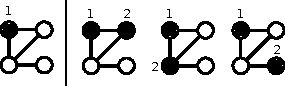
\includegraphics[scale=1.5]{labelling_ext_example.pdf}
    \caption{All possible label extensions of a flag}
    \label{fig:labelling_ext_example}
\end{figure}

The other technicality we need to address is that of the hereditary nature of graph
classes. In the classic flag algebra we always assumed that $\Gcl$ was hereditary. We want
to be able to talk about some non-hereditary graph classes $\Gcl$. This is not a major
obstacle but means we need to adjust our notation.

\begin{definition}[Hereditary Closure]
    Given a graph class $\Gcl$ we define the \textbf{hereditary closure} of $\Gcl$ to be
    the smallest graph class which contains $\Gcl$ and is closed under taking
    induced subgraphs. i.e. it's the graphs $G\in\Gcl$ with their induced subgraphs.

    We denote this as $\HeredG$.
\end{definition}

Now we are ready to define our local flags:

\begin{definition}[Local $\sigma$-Flag]
    \label{def:local_flag}
    Fix some graph class $\Gcl$ and takes its hereditary closure $\HeredG$.
    Let $\sigma$ be a type. Then a $\sigma$-flag $(F, \theta)\in\HeredG{}^\sigma$ is a
    \textbf{local $\sigma$-flag} if we have the following properties:
    \begin{enumerate}
        \item $(G,\eta) \to \rho((F,\theta); (G,\eta))$ is a bounded function as a function
            $\Gcl^\sigma\to\R_{\geq 0}$. (We are very intentionally using $\Gcl$ and not its closure here).
        \item If we label any of $F$'s unlabelled vertices we get another local flag.
    \end{enumerate}
\end{definition}

To state this 2nd property more precisely: We require that for any label extension
$\theta'$ of $\theta$, the induced extended flag $(F,\theta')$ is also a local flag.
This is not a circular definition as any label extension of $(F,\theta)$ reduces the number of
unlabelled vertices
by 1; We could define inductively starting with those flags with no unlabelled vertices.

What we're trying to capture here is that any "subflag" of $F$ is also a local flag, meaning we can
pin down $F$'s vertices and continue to get bounded behaviour.

\begin{example}
    As in the example above $F=\edgemarked$ gives rise to a bounded local
    density function $\rho$. The only label extension of $F$ is the edge
    with both vertices labelled $F' = \edgebothmarked$. This (as with all flags with no
    unlabelled vertices) has $c(F'; G) = 1$ so $\rho(F; G) = 1/\binom{\Delta(G)}{0}=1$
    which is bounded so $F'$ is a local flag. Hence $F=\edgemarked$ is a local flag.
\end{example}

We write $\Glocn^\sigma\subseteq\HeredG{}^\sigma_n$ for the set of local $\sigma$-flags
of size $n$ up to isomorphism, and $\Gloc^\sigma$ for all local $\sigma$-flags. As usual we
can drop the $\sigma$ superscript if $\sigma=\emptyset$.

\begin{note}
    For $\sigma$-flag $F$ the requirement that $\rho(F; G)$ is a bounded function
    is equivalent to requiring that $c(F; G) \in O(\Delta(G)^{|F|-|\sigma|})$.
\end{note}

Comparing this section to the classic flag algebra case (section \ref{sec:flag_algebras})
you might expect us to introduce something akin to the chain rule (lemma \ref{lemma:chain_rule}).
Unfortunately no such relation exists in general for local flags. This is the first big
loss when moving to the new framework: Prima facie it's unclear how one can "project"
small flags into the space of larger flags.

\begin{note}
    This second property we require of local flags is not necessarily implied by
    the first which we show now in lemma \ref{lemma:second_prop_required}.
\end{note}

\begin{lemma}
    \label{lemma:second_prop_required}
    There is a class of graphs $\Gcl$ and $\sigma$-flag $F$ such that
    $G \mapsto \rho(F; G)$ is a bounded function $\Gcl^\sigma \to \R$ but $F$ is
    not a local $\sigma$-flag. i.e. $F$ has a labelled extension with unbounded
    density function.
\end{lemma}
\begin{proof}
    Take $\Gcl$ to be the class of 3-vertex-coloured graphs (black, red and blue) $G$
    which have a single red vertex and $\Delta(G)^2$ blue vertices\footnote{Implicitly the
    rest of the vertices are black} such that there are no edges between red and blue
    vertices.

    Then take $\emptyset$-flag $F=\redbluenonedge$. For any $G\in\Gcl$ we have
    $c(F; G) = \Delta(G)^2$ as there is 1 choice for the red vertex and $\Delta(G)^2$
    choices for the blue. Hence $\rho(F;G) = c(F; G) / \binom{\Delta(G)}{2} \leq 2$.
    Consider then the labelled extension $F' =\redbluenonedgemarked$ of type
    $\redvertex$. We have $c(F'; G)=\Delta(G)^2$ again for any
    $G\in\Gcl^\redvertex$ but now $\rho(F'; G) = \Delta(G)^2 / \Delta(G) = \Delta(G)$ which
    is an unbounded function. Hence $F'$ is not a local $\redvertex$-flag
    meaning $F$ is not a local $\emptyset$-flag.
\end{proof}

Intuitively $F$ is a local $\sigma$-flag (relative to our choice of $\Gcl$ and
$\Delta$) if $\Delta(G)$ bounds the "degree of freedom" for the possible mapping
of $F$'s unlabelled vertices.

\begin{lemma}
    \label{lemma:local_if_connected}
    If $\Delta(G)$ is the max degree function then any $\sigma$-flag $F$ is a
    local $\sigma$-flag if all connected components of $F$ contains a labelled
    vertex.
\end{lemma}

\begin{proof}
    Intuitively the labelled vertices are fixed. The vertices directly connected to
    labelled vertices have $\Delta(G)$ choices. After mapping those we again have
    $\Delta(G)$ choices for their unmapped neighbours etc leading to a total
    bound of $O(\Delta(G)^{|F|-|\sigma|})$ choices.

    The full details of the proof can be found in the proof of
    lemma \ref{lemma:pentagon_local_flags}.
\end{proof}

\section{Algebraic Structure}

Now that we have described local $\sigma$-flags $\Gloc^\sigma$ we can describe their
algebraic structure. Ideally we would like to construct a product structure
on $\Gloc^\sigma$ such that we get a result like theorem \ref{thm:classic_product_lim} but for
the local density function $\rho$. In fact this is exactly what we get: An algebraic structure such
that $\rho(f; G)\rho(g;G) = \rho(f\cdot g; G) + o(1)$ (Theorem \ref{thm:local_product_lim}).

First we take the concept of limit functionals (section \ref{sec:limit_functionals})
from the classic flag algebras with some minor modifications:
First, we require now that a sequence of graphs $(G_k)_{k\in\N}$ is $\Delta$-increasing:
\begin{definition}
    A sequence $(G_k)_{k\in\N}$ is $\Delta$-increasing if the sequence
    $(\Delta(G))_{k\in\N}$ is strictly increasing\footnote{We required that the codomain of
    $\Delta$ was $\N$ so strictly increasing implies unbounded. Generalising $\Delta$
    to a function with codomain $\R$ is likely possible so we would need to add the
    unbounded requirement here.}.
\end{definition}
Then given some $\Delta$-increasing sequence of $\sigma$-flags $(G_k)_{k\in\N}$
and some local $\sigma$-flag
$F$ we can look at $\lim_{k\to\infty}\rho(F; G_k)$. As $F$ is a local $\sigma$-flag
$\rho(F; \cdot)$ is bounded so the image is compact. For this reason (again via Tychonoff's theorem)
any sequence of $\sigma$-flags $(G_k)_{k\in\N}$ contains a convergent subsequence meaning
$\lim_{k\to\infty}\rho(F; G_k)$ exists for all $F\in\Gloc^\sigma$.
Hence we can define a limit functional $\phi\colon\Gloc^\sigma\to\R$
from such a convergent sequence $(G_k)_{k\in\N}$ as $\phi(F):=\lim_{k\to\infty}\rho(F; G_k)$.

As with the classic case we can take the space of formal linear combinations of
local flags $\R\Gloc^\sigma$ and linearly extend $\rho$ and $\phi$ to these
spaces. As before we denote the set of all limit functionals on type $\sigma$ by
$\Phi^\sigma$.

\begin{note}
    Unlike in the classic case we will not be quotienting the space $\R\Gloc^\sigma$ by
    a subspace. This is as we do not have an equivalent relation to the chain rule.
    The side effect of this is that there may be vectors $f \in \R\Gloc^\sigma$ which
    are formally non-zero but have $\phi(f) = 0\ \forall\ \phi\in\Phi^\sigma$.
    This doesn't affect the correctness of our arguments, but does mean the semidefinite
    programs will be larger and therefore may take longer to solve.
\end{note}

We now define the product on $\R\Gloc^\sigma$ which will turn it into an algebra.

\begin{definition}[Local Flag Product]
    Let $F, F'\in\Gloc^\sigma$ be given. Let $n=|F|+|F'|-|\sigma|$, the minimum size of
    a flag which can fit $F$ and $F'$. Then we define:
    \[
        F \cdot F' := \sum_{H \in \Glocn^\sigma} p(F, F'; H) \cdot H
    \]
    Note: This is the induced density function $p$, not the local density function $\rho$.
    Extend this product bilinearly to the space $\R\Gloc^\sigma$ to create an algebra
    $\Lcl^\sigma$.
\end{definition}

\begin{note}
    It will be useful in later chapters to refer to the subspace of $\Lcl^\sigma$
    spanned by flags of a fixed size $n$. Call this subspace $\Lcl^\sigma_n$.
\end{note}

This product has the exact limiting behaviour that we need and some nice algebraic
properties:

\begin{theorem}
    \label{thm:local_product_lim}
    For $f, g \in \Lcl^\sigma$ and $\sigma$-flag $G$ we have
    \[\rho(f; G)\rho(g; G) = \rho(f\cdot g; G) + O\left(\frac{1}{\Delta(G)}\right)\]
    and in particular any limit functional $\phi\in\Phi^\sigma$ is an algebra
    homomorphism $\Lcl^\sigma \to \R$.
\end{theorem}

\begin{lemma}
    \label{lemma:local_assoc}
    The algebra $\Lcl^\sigma$ is commutative, associative and unital.
\end{lemma}

We will prove both of these results after first proving a key technical result which makes this
product work:

\begin{theorem}
    Let $F, F' \in \Gloc^\sigma$ be local $\sigma$-flags and $H$ a $\sigma$-flag
    of size $n=|F|+|F'|-|\sigma|$ such that $p(F, F'; H) > 0$ then $H$ is a local
    $\sigma$-flag.
\end{theorem}

\begin{proof}
    Let $\theta,\theta'$ be the $\sigma$ embeddings for $F, F'$ and $\eta$ the
    $\sigma$-embedding for $H.$
    To prove $H$ is a local flag we first need to show that $\rho(H; \cdot)$ is a bounded function.
    i.e. $(G \mapsto c(H; G)) \in O(\Delta(G)^{|H|-|\sigma|}).$

    As $p(F, F'; H) > 0$ there is some $U, U'\subseteq V(H)$ such that $U\cap U'=\im\eta$ and
    $F \cong H[U] \land F'\cong H[U']$ as $\sigma$ flags. As $|H|=|F|+|F'|-|\sigma$ we
    have $U \cup U' = V(H)$.

    Let $(G, \zeta)$ be another $\sigma$-flag. If $c(H; G) = 0$ we're done so assume otherwise and
    let $\im\zeta \subseteq V\subseteq V(G)$ be such that $H \cong G[V]$ as $\sigma$-flags. Let
    $\phi$ be this isomorphism. Then In particular $\phi$ induces an embedding of $U, U'$ into
    $V(G)$ such that $\im\zeta = \phi(U) \cap \phi(U')$ and $G[\phi(U)] \cong F\land G[\phi(U')]
    \cong F'$ as $\sigma$-flags.  Hence any choice of an instance of $H$ in $G$ and choice of
    instances $U, U'$ of $F, F'$ in $H$ gives rise to a pair of instances of $F$ and $F'$ in $G.$
    There are at most some constant number $C$ instances of $F, F'$ in $H$ (as the size of $H$ is
    fixed).

    Note then also that any choice of a pair of instances of $F, F'$ in $G$ can be derived from at
    most 1 instance of $H$, as the size of $H$ was chosen to be the minimum possible such that both
    $F,F'$ fit. If the two instances overlap (outside of the required intersection at $\im\zeta$)
    then they don't correspond to an instance of $H.$ If they don't overlap then their
    union corresponds to a single \textit{possible} instance of $H$.

    In summary each instance of $H$ gives rise to some non-zero but bounded number of pairs of
    instances of $F, F'$ in $G$, and each pair of instances of $F, F'$ is induced by at most
    1 instance of $H.$
    Therefore $c(H; G) \leq \frac{1}{C}\cdot c(F; G)\cdot c(F'; G)$. We use then
    the fact that $F$ and $F'$ are local $\sigma$-flags so $c(F; \cdot)$ and
    $c(F'; \cdot)$ are $\in O(\Delta(G)^{|F|-|\sigma|})$ and $\in O(\Delta(G)^{|F'|-|\sigma|})$
    respectively. Hence their product is
    $\in O(\Delta(G)^{|F|+|F'|-2|\sigma|}) = O(\Delta(G)^{|H|-|\sigma|})$ so
    $c(H; \cdot) \in O(\Delta(G)^{|H|-|\sigma|})$ showing $\rho(H; \cdot)$ is a bounded function as
    required.

    \begin{figure}[!ht]
        \centering
        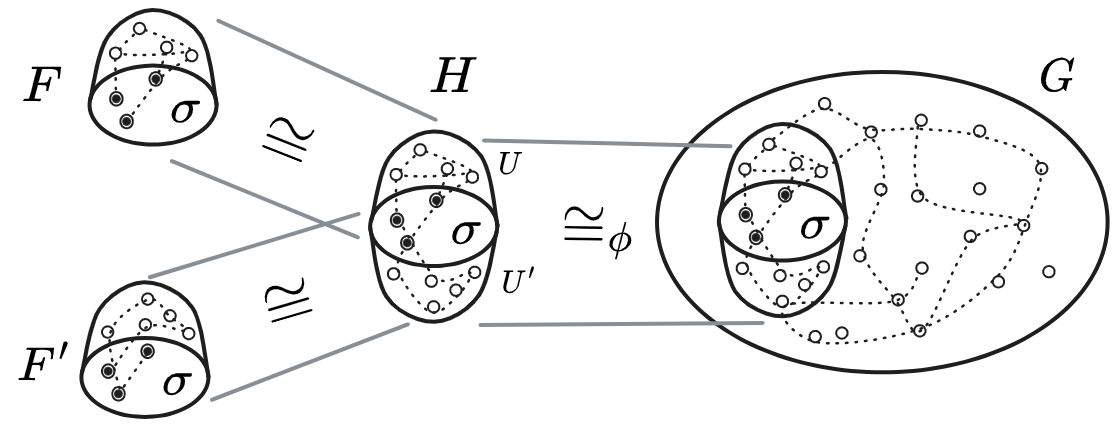
\includegraphics[scale=0.25]{local_flag_product_diagram}
    \end{figure}

    It remains to prove that $H$ still has bounded density after fixing any unlabelled vertices.
    This argument goes almost identically so I just give the high level details. Once again
    pick $U, U' \subseteq V(H)$ where $U\cap U'=\im\eta$ and $F\cong H[U]$ and $F' \cong H[U']$.
    Pick some unlabelled vertex $v\in V(H)\setminus \im\eta$.
    Let $H^v$ be the labelled extension fixing $v$. Then any copy of $H^v$ in $G$ induces
    via $U, U'$ copies of $F, F'$ in $G$. WLOG $v \in U \setminus \im \eta$ so each copy
    of $F$ induced by $U$ is also a copy of $F^v$, the labelled extension of $f$ fixing the
    preimage of $v$. Then as $F$ is local $F^v$ has bounded corresponding density
    function. Once again we have some constant $C$ number of choices for $U, U'$ so we
    get
    $c(H^v; G) \leq \frac{1}{C} c(F^v; G) \cdot c(F'; G) \in
    O(\Delta(G)^{|F|-(|\sigma|+1)+|F'|-|\sigma|}) = O(\Delta(G)^{|H|-(|\sigma|+1)})$
    as required.  $\therefore H$ is a local flag.
\end{proof}

The value of this theorem is that it tells us that our local product definition is
equivalent to summing over all $\sigma$-flags, not just the local flags:

\begin{corollary}
    \label{corollary:local_product}
    For local flags $F, F' \in \Gloc^\sigma$ we have
    \[
        F \cdot_{\Lcl^\sigma} F'
        = \sum_{H\in\Glocn^\sigma}p(F, F'; H)\cdot H
        = \sum_{H\in\Gcl_n^\sigma}p(F, F'; H)\cdot H
    \]
    where $n=|F|+|F'|-|\sigma|$.
\end{corollary}

This allows us to prove our product limiting result (Theorem \ref{thm:local_product_lim}).

\begin{proof}[Proof of theorem \ref{thm:local_product_lim}]
    Let $(F,\theta), (F',\theta') \in\Gloc^\sigma$ be local $\sigma$-flags and $(G,\eta)$ a
    $\sigma$-flag. We compute
    \[
        \begin{split}
            \rho(F; G)\cdot\rho(F';G) -\rho(F\cdot F'; G)
            &= \rho(F; G)\cdot\rho(F';G)
                - \left(\sum_{H\in\Glocn^\sigma} p(F, F'; H)\rho(H; G) \right)\\
            &= \rho(F; G)\cdot\rho(F';G)
                - \left(\sum_{H\in\Gcl_n^\sigma} p(F, F'; H)\rho(H; G) \right)\\
            &= \frac{c(F; G)\cdot c(F';G)}{\binom{\Delta(G)}{|F|-k}\binom{\Delta(G)}{|F'|-k}}
                - \frac{\sum_{H\in\Gcl^\sigma_n} c(F, F'; H)c(H; G)}
                {\binom{n-k}{|F|-k}\binom{\Delta(G)}{n-k}}
            \end{split}
    \]
    where $k=|\sigma|$ and $n=|F|+|F'|-k$.
    First we note the denominators are asymptotically equivalent. It is a standard
    binomial identity that
    $\binom{\Delta(G)}{n-k}\binom{n-k}{|F|-k} = \binom{\Delta(G)}{|F|-k}\binom{\Delta(G)-(|F|-k)}{|F'|-k}$
    hence
    \[
        \lim_{\Delta(G)\to\infty}
        \frac{\binom{n-k}{|F|-k}\binom{\Delta(G)}{n-k}}{\binom{\Delta(G)}{|F|-k}\binom{\Delta(G)}{|F'|-k}}
        = \lim_{\Delta(G)\to\infty}
        \frac{\binom{\Delta(G)}{|F'|-k}}{\binom{\Delta(G)-(|F|-k)}{|F'|-k}}
        = 1.
    \]
    Both denominators are asymptotically equivalent and $\in\Omega(\Delta(G)^{n-k})$ so we
    can focus on the numerators:
    \[
        c(F;G)c(F';G) - \sum_{H\in\Gcl^\sigma_n}c(F,F';H)c(H;G).
        \tag{$\dagger$}
    \]
    It suffices to show $(\dagger) \in O(\Delta(G)^{n-k-1})$.

    The term $c(F; G)c(F';G)$ counts the number of pairs of subsets
    $\im\eta \subseteq U, U' \subseteq V(G)$ such that $F \cong G[U]$ and $F'\cong G[U']$.
    Comparatively the sum $\sum_{H\in\Gcl^\sigma_n} c(F, F'; H)c(H; G)$ counts the number
    of subsets $\im\eta U, U' \in V(G)$ such that $F\cong G[U]$, $F'\cong G[U']$ \textit{and}
    $U \cap U' = \im \eta$. This relies on theorem \ref{thm:local_product_lim}
    which let us sum over all possible flags of size $n$.

    Clearly then ($\dagger$) counts the
    number of pairs of subsets $\im\eta \subseteq U, U' \subseteq V(G)$ such that
    $F \cong G[U], F'\cong G[U']$ and $U \cap U' \neq \im \eta$ meaning there is
    an overlap of the image of the unlabelled vertices of $F, F'$.

    To see intuitively that $(\dagger)\in O(\Delta(G)^{n-k-1})$
    remember that $F,F'$ being local flags means $\Delta(G)$
    bounds the degree of freedom of choosing the image of each of their unlabelled vertices.
    Then $\Delta(G)^{n-k}$ represents the degree
    of freedom of choosing pairs of embeddings of $F, F'$ with no constraints; Adding
    the constraint that the embeddings must overlap means reducing the degree of freedom
    by at least one, giving $\Delta(G)^{n-k-1}$. We show the argument in detail here:

    We calculate an upper bound on ($\dagger$) by summing for each $U$ embedding $F$ into $G$
    and over each unlabelled $v \in V(F)$ the maximum number of $U'$ embeddings of $F'$ which
    overlap on the image of $v$.

    Fix $\im\eta\subseteq U \subseteq V(G)$ such that $F \cong G[U]$ and
    $v\in V(F) \setminus \im\eta$. Call the isomorphism $\phi$. We ask then
    how many $\im\eta \subseteq U' \subseteq V(G)$ are there such that $\phi(v)\in U'$ and
    $F' \cong G[U']$? We can upper bound this by summing over each unlabelled
    $w \in V(F')$ and asking how many $U'$ embeddings are there where the isomorphism
    maps $w$ to $\phi(v)$.
    This is exactly what is answered by taking a labelled extension of $F'$ labelling
    $w$ and extending the label of $G$ to map $w$ to $\phi(v)$. We are guaranteed that
    $F'$ is a local flag so this labelled extension also has bounded density. In particular
    $c((F')^w; G^{\phi(v)})\in O(\Delta(G)^{|F'|-(k+1)})$.

    \begin{figure}[!ht]
        \centering
        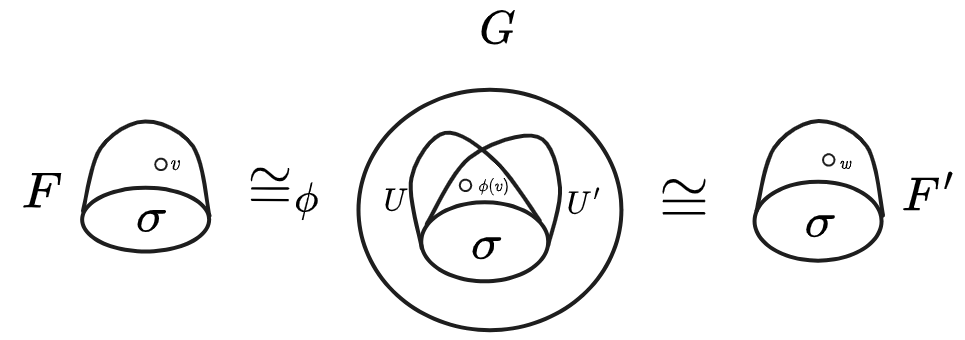
\includegraphics[scale=0.25]{local_flag_limit_diagram}
    \end{figure}

    We have a constant number of choices of $w$ and $v$ and $c(F; G) \in O(\Delta(G)^{|F|-k})$
    choices for $U$ giving us a total upper bound of
    $O(\Delta(G)^{|F|-k + |F'|-(k+1)}) = O(\Delta(G)^{n-k-1})$ as required.
    \[
        \therefore \rho(F; G)\rho(F'; G) - \rho(F\cdot F'; G)
        = \frac{O(\Delta(G)^{n-k-1})}{\Omega(\Delta(G)^{n-k})}
        = O\left(\frac{1}{\Delta(G)}\right).
    \]
    This then extends linearly to $\Lcl^\sigma = \R\Gloc^\sigma$ as
    the vector space only contains finite combinations.
    This has the immediate corollary of showing that any limit functional
    $\phi\in\Phi^\sigma$ is an algebra homomorphism $\Lcl^\sigma \to \R$.
\end{proof}

Finally we can prove lemma \ref{lemma:local_assoc}, showing $\Lcl^\sigma$ to be associative,
commutative and unital.

\begin{proof}[Proof of Lemma \ref{lemma:local_assoc}]
    It is clear by definition that the product is commutative.

    To show associativity let $F_1, F_2, F_3$ be local $\sigma$-flags.
    Then let $k = |\sigma|, \ell = |F_1|+|F_2|-k$ and $n = |F_1|+|F_2|+|F_3|-2k$. Then
    we can calculate:

    \[
        \begin{split}
            (F_1 \cdot F_2) \cdot F_3
            &= \left(\sum_{H\in\Glocsub{\ell}^\sigma} p(F_1,F_2;H)H\right) \cdot F_3\\
            &= \left(\sum_{H\in\Gcl_\ell^\sigma} p(F_1,F_2;H)H\right) \cdot F_3\\
            &= \sum_{H\in\Gcl_\ell^\sigma} p(F_1,F_2;H)(H \cdot F_3)\\
            &= \sum_{H\in\Gcl_\ell^\sigma} p(F_1,F_2;H)
                \left(\sum_{G\in\Glocn^\sigma} p(H,F_3;G)G \right)\\
            &= \sum_{G\in\Glocn^\sigma}
                \left(\sum_{H\in\Gcl_\ell^\sigma} p(F_1,F_2;H) p(H,F_3;G) \right) G
        \end{split}
    \]
    Then as we used our previous lemma to get a sum over all flags, not just local ones, we can
    apply the chain rule for induced densities (lemma \ref{lemma:chain_rule})
    to get:
    \[
            (F_1 \cdot F_2) \cdot F_3
            = \sum_{G\in\Glocn^\sigma} p(F_1, F_2, F_3; G)\cdot G
    \]
    This is symmetric in all 3 terms so clearly $(F_1\cdot F_2)\cdot F_3 = F_1 \cdot (F_2\cdot F_3)$
    so $\Lcl^\sigma$ is associative.

    Finally take the type $\sigma$ and view it as a $\sigma$-flag implicitly. Then
    $c(\sigma; G)=1$ for any $\sigma$-flag $G$ so $\rho(\sigma; G)=1/\binom{\Delta(G)}{0}=1$
    showing $\sigma$ is a local $\sigma$-flag $\implies \sigma\in\Lcl^\sigma$.
    Then it is easy to see that $\sigma$ is a unit in this algebra as for any
    $F\in\Lcl^\sigma$ we have
    $F\cdot\sigma = \sum_{H \in \Glocsub{|F|}^\sigma}p(F,\sigma; H)H=F$
    as the only flag of size $|F|$ which contains a copy of $F$ is $F$ itself.
\end{proof}

\section{Positivity}

We previously adopted the idea of limit functionals almost directly from the
classic flag algebra, we now do the same with positivity. 
\begin{definition}[Positive Element]
    We say $f\in\Lcl^\sigma$ is a positive element, denoted $f \geq_{\Lcl^\sigma} 0$ or
    just $f\geq 0$, if $\phi(f) \geq 0\ \forall \phi\in\Phi^\sigma$.
\end{definition} 

We then denote the convex cone of all positive elements of $\Lcl^\sigma$ by
$\SemCone^\sigma$. We again call this the (local) semantic cone.

\section{Averaging Local Flags}

So far we have made restrictions no restrictions on what types $\sigma$ we consider, but
it will prove useful to look at only a select set of types we call \textit{local types}.
\begin{definition}[Local Type]
    We say that a type (definition \ref{def:type}) is a \textbf{local type}
    if $\downflag{F}$ is a local $\emptyset$-flag for all $F\in\Gloc^\sigma$.
\end{definition}

We also give a useful equivalent condition:
\begin{lemma}
    \label{lemma:local_type_equiv}
    A type $\sigma$ is a local type iff $\sigma$ is itself a local $\emptyset$-flag
\end{lemma}

\begin{proof}
    One direction is easy to see. If $\sigma$ is a local type then as $\sigma\in\Gloc^\sigma$
    we have $\downflag{\sigma}\in\Gloc^\emptyset$ but $\downflag{\sigma}=\sigma$ so
    $\sigma$ is a local $\emptyset$-flag.

    To show the other direction assume $\sigma$ is itself a local $\emptyset$-flag
    meaning $c(\sigma; G) \in O(\Delta(G)^{|\sigma|})$. Let $(F, \theta) \in\Gloc^\sigma$ be
    given, then we also have\\
    $c((F, \theta); (G, \eta)) \in O(\Delta(G)^{|F|-|\sigma|})$.
    Let $C_\sigma$ be the constant such that\\
    $c(\sigma; G) \leq C_\sigma \Delta(G)^{|\sigma|}\forall G\in\Gcl$ and
    $C_F^\sigma$ the constant such that\\
    $c((F, \theta); (G, \eta)) \leq C_F^\sigma\Delta(G)^{|F|-|\sigma|}\forall
    (G,\eta)\in\Gcl^\sigma$. For fixed $\sigma$ and $U \subseteq V(G)$ there is
    a finite number of possible embeddings $\eta$ such that $(G,\eta)$ is a
    $\sigma$-embedding and $\im\eta=U$, namely the size of the automorphism group of $\sigma$
    $|\mathrm{Aut}(\sigma)|$.

    We want to show that $\downflag{(F,\theta)}=F$ is a local $\emptyset$-flag so first need to show
    $c(F; G) \in O(\Delta(G)^{|F|})$.
    Given any embedding $(G,\eta)$ and $\im\eta \subseteq U \subseteq V(G)$ such that
    $(F,\theta) \cong (G[U],\eta)$ we must have $F \cong G[U]$ as $\emptyset$-graphs.
    This gives us a map into copies of $F$ in $G$ which is just forgetting the labels
    in both $(G,\eta)$ and $(F,\theta)$.
    Conversely consider some copy of $F$ in $G$ $U \subseteq V(G)$ ($F \cong G[U]$ as
    $\emptyset$-flags). Then as $(F,\theta)$ is a $\sigma$-flag there is some $V\subseteq U$ such
    that $\sigma \cong G[V]$. We can then construct a $\sigma$-flag $(G,\eta)$ where
    $\im\eta=V$ such that $(F, \theta) \cong (G[U], \eta)$ as $\sigma$-flags.
    This shows us that the previous map must be surjective.
    Hence
    \[
        \begin{split}
            c(F; G)
            &\leq \left|\{ ((G, \eta), U)\colon
                \im\eta \subseteq U \subseteq V(G)\ \text{such that}\ (F,\theta) \cong (G[U],\eta)
                \}\right|\\
            &\leq \sum_{(G,\eta)\in\Gcl^\sigma}
                \left|\{ U\colon
                \im\eta \subseteq U \subseteq V(G)\ \text{such that}\ (F,\theta) \cong (G[U],\eta)
                \}\right|\\
            &\leq \sum_{(G,\eta)\in\Gcl^\sigma} c((F,\theta), (G,\eta))\\
            &\leq \sum_{(G,\eta)\in\Gcl^\sigma} C_F^\sigma\Delta(G)^{|F|-|\sigma|}\\
            &\leq |\mathrm{Aut}(\sigma)|c(\sigma; G) C_F^\sigma\Delta(G)^{|F|-|\sigma|}\\
            &\leq |\mathrm{Aut}(\sigma)|C_\sigma\Delta(G)^{|\sigma|} C_F^\sigma\Delta(G)^{|F|-|\sigma|}\\
            &\in O(\Delta(G)^{|F|})
        \end{split}
    \]
    as required. It remains to show that any labelled extension of $\downflag{F}$
    also has bounded density function. $\downflag{F}$ is an $\emptyset$-flag so
    a labelled extension $F'$ of $\downflag{F}$ is just $F$ with a single labelled vertex.
    There are 2 cases but they both proceed similarly. If this labelled
    vertex is in $\im\theta\subseteq V(F)$ then as $\sigma$ is a local $\emptyset$-flag
    by an almost identical argument to the previous we get a bound of
    $c(F'; G^v) \in O(\Delta(G)^{|F|-1})$. The other case is that the newly labelled
    vertex of $\downflag{F}$ is one of the unlabelled vertices in $F$, in which case
    we use that $F$ is a local $\sigma$-flag to again bound
    $c(F'; G^v) \in O(\Delta(G)^{|F|-1})$ as required.
    Therefore $\downflag{F}$ is a local $\emptyset$-flag.
\end{proof}

We adopt this definition of local type because we would like to introduce an averaging
operator $\llbracket \cdot \rrbracket \colon \Lcl^\sigma \to \Lcl^\emptyset$ akin
to definition \ref{def:classic_averaging} but we cannot just apply this map directly
as we don't generally have a guarantee that $\llbracket f \rrbracket \in \Lcl^\emptyset$ even
if $f\in\Lcl^\sigma$. By our definition above this map is well
defined if $\sigma$ is local type.

\begin{definition}[Averaging operator]
    As a reminder we have a normalisation function $q_\sigma\colon\Gcl^\sigma\to[0, 1]$
    given in definition \ref{def:averaging_normalisation}.
    Define the \textbf{averaging operator}
    $\llbracket \cdot \rrbracket\colon \R\Gcl^\sigma \to \R\Gcl^\emptyset$
    as before by defining
    $\llbracket F \rrbracket = q_\sigma(F)\downflag{F}$ for $F\in\Gcl^\sigma$ and
    extend linearly.

    If $\sigma$ is a local type and we restrict the domain to $\R\Gloc^\sigma = \Lcl^\sigma$
    we get a map
    $\llbracket \cdot\rrbracket\colon \Lcl^\sigma \to \Lcl^\emptyset$.
\end{definition}

We have a very nice result (lemma \ref{lemma:classic_exp_flags}) in the classic case where this
operator represents an average in a very concrete way:
$\E_\theta[p(F; (G,\theta))] = \frac{p(\llbracket F \rrbracket; G)}{p(\llbracket\sigma\rrbracket;
G)}$
We do not get quite such a neat relation for local densities, but we do get the relation
in the limit:

\begin{lemma}
    \label{lemma:local_averaging_exp}
    For $\sigma$-flag $F$ and graph ($\emptyset$-flag) $G\in\Gcl$ we have
    \[
        \E_\theta[\rho(F; (G,\theta))] \sim
        \frac{\rho(\llbracket F\rrbracket; G)}{\rho(\llbracket \sigma\rrbracket; G)}
        \ \text{as}\ \Delta(G) \to \infty
    \]
    where $\theta$ is a uniformly random $\sigma$-embedding into $G$.
\end{lemma}

\begin{proof}
    This proof uses the fact that this relation holds for induced densities
    (lemma \ref{lemma:classic_exp_flags}) and the following relation between
    induced and local densities:
    For any $\sigma$-flags $H$ and $G$ we have
    \[
        \rho(H; G)
        = \frac{c(H; G)}{\binom{\Delta(G)}{|H|-|\sigma|}}
        = \frac{\binom{|G|-|\sigma|}{|H|-|\sigma|}c(H;
        G)}{\binom{|G|-|\sigma|}{|H|-|\sigma|}\binom{\Delta(G)}{|H|-|\sigma|}}
        =
        \frac{\binom{|G|-|\sigma|}{|H|-|\sigma|}}{\binom{\Delta(G)}{|H|-|\sigma|}}\frac{c(H;G)}{\binom{|G|-|\sigma|}{|H|-|\sigma|}}
        = \frac{\binom{|G|-|\sigma|}{|H|-|\sigma|}}{\binom{\Delta(G)}{|H|-|\sigma|}}p(H;G)
    \]
    Therefore
    \[
        \frac{\rho(\llbracket F\rrbracket; G)}
        {\rho(\llbracket \sigma\rrbracket; G)}
        =
        \frac{p(\llbracket F\rrbracket; G)}
        {p(\llbracket \sigma\rrbracket; G)}
        \frac{\binom{|G|}{|F|}}{\binom{\Delta(G)}{|F|}}
        \frac{\binom{\Delta(G)}{|\sigma|}}{\binom{|G|}{|\sigma|}}.
    \]
    Now we use lemma \ref{lemma:classic_exp_flags} to show
    \[
        \begin{split}
            \frac{\rho(\llbracket F\rrbracket; G)}
            {\rho(\llbracket \sigma\rrbracket; G)}
            &= \E_\theta[p(F; (G,\theta))]
            \frac{\binom{|G|}{|F|}}{\binom{\Delta(G)}{|F|}}
            \frac{\binom{\Delta(G)}{|\sigma|}}{\binom{|G|}{|\sigma|}}\\
            &= \E_\theta[\rho(F; (G,\theta))]
            \frac{\binom{\Delta(G)}{|F|-|\sigma|}}{\binom{|G|-|\sigma|}{|F|-|\sigma|}}
            \frac{\binom{|G|}{|F|}}{\binom{\Delta(G)}{|F|}}
            \frac{\binom{\Delta(G)}{|\sigma|}}{\binom{|G|}{|\sigma|}}\\
            &= \E_\theta[\rho(F; (G,\theta))]
            \frac{\binom{\Delta(G)}{|F|-|\sigma|}\binom{\Delta(G)}{|\sigma|}}
            {\binom{\Delta(G)}{|F|}}
            \frac{\binom{|G|}{|F|}}
            {\binom{|G|-|\sigma|}{|F|-|\sigma|}\binom{|G|}{|\sigma|}}
        \end{split}
    \]
    We can use standard binomial relations to reduce this to
    \[
        \frac{\rho(\llbracket F\rrbracket; G)}
        {\rho(\llbracket \sigma\rrbracket; G)}
        = \E_\theta[\rho(F; (G,\theta))]
        \frac{\binom{\Delta(G)}{|F|-|\sigma|}\binom{\Delta(G)}{|\sigma|}}
        {\binom{\Delta(G)}{|F|}\binom{|F|}{|\sigma|}}
        = \E_\theta[\rho(F; (G,\theta))]
        \frac{\binom{\Delta(G)}{|F|-|\sigma|}}
        {\binom{\Delta(G)-|\sigma|}{|F|-|\sigma|}}
    \]
    Then
    $\lim_{\Delta(G)\to\infty}\binom{\Delta(G)}{|F|-|\sigma|}/\binom{\Delta(G)-|\sigma|}{|F|-|\sigma|}
    = 1$ so we do indeed get
    \[
        \frac{\rho(\llbracket F\rrbracket; G)}
        {\rho(\llbracket \sigma\rrbracket; G)}
        = (1+o(1)) \E_\theta[\rho(F; (G,\theta))]
        \implies
        \frac{\rho(\llbracket F\rrbracket; G)}
        {\rho(\llbracket \sigma\rrbracket; G)}
        \sim \E_\theta[\rho(F; (G,\theta))].
    \]
\end{proof}

Now we can show that the averaging operator preserves positivity as in the
classic case (lemma \ref{lemma:classic_pos_preserve}). We only get this
behaviour if $\sigma$ is a local type.

\begin{lemma}
    \label{lemma:local_pos_preserve}
    Let $\sigma$ be a local type. Then the averaging operator preserves positive
    elements of $\Lcl^\sigma$:
    $\llbracket \SemCone^\sigma \rrbracket \subseteq  \SemCone^\emptyset$.
    In particular as with the classic case we have $\llbracket f^2 \rrbracket \geq 0$
    for all $f\in\Lcl^\sigma$.
\end{lemma}

\begin{proof}
    As $\sigma$ is a local type we have that
    $\llbracket \SemCone^\sigma \rrbracket \subseteq \Lcl^\emptyset$.

    Let $f\in\SemCone^\sigma$ be given and assume for sake of contradiction that
    $\llbracket f \rrbracket \notin\SemCone^\emptyset$. Then there must exist
    some limit functional $\phi\in\Phi^\emptyset$ such that $\phi(f)<0$. Equivalently
    there is some $\Delta$-convergent sequence of graphs $(G_k)_{k\in\N}$
    such that $\lim_{k\to\infty}\rho(f; G_k) < 0$.

    By lemma \ref{lemma:local_averaging_exp} we know that
    \[
        \rho(\llbracket f\rrbracket; G_k) = (1+o(1)) \rho(\llbracket \sigma \rrbracket; G_k)
        \E_\theta[\rho(f; (G_k,\theta))]
    \]
    where $o(1)$ is as $k \to \infty$.
    In particular this means we must have
    \[
        \lim_{k\to\infty} \rho(\llbracket \sigma \rrbracket; G_k)
        \E_\theta[\rho(f; (G_k,\theta))] < 0.
    \]
    Then as $\sigma$ is a local type $\sigma$ is a local $\emptyset$-flag so has bounded
    density: $\exists$ a constant $C$ such that $C \geq \rho(\llbracket\sigma\rrbracket; G_k) \geq
    0\forall k\in\N$. In particular then we must have
    \[
        \lim_{k\to\infty} \E_\theta[\rho(f; (G_k,\theta))] < 0.
    \]
    Therefore there is some $k_0$ large enough such that
    $\E_\theta[\rho(f; (G_k, \theta))] < 0\ \forall\ k \geq k_0$. In particular then
    for each $k \geq k_0$ by the properties of the expected value there must exist
    some $\sigma$-embedding $\theta_k$ such that
    $\rho(f; (G_k, \theta_k)) \leq \E_\theta[\rho(f; (G_k,\theta))] < 0$. This gives
    us a $\Delta$-increasing sequence of $\sigma$-flags which must contain a convergent
    subsequence $(G'_k, \theta'_k)_{k\in\N}$
    which in turn gives us a limit functional $\phi\in\Phi^\sigma$. This limit functional
    then must have the property that
    \[
        \phi(f) = \lim_{k\to\infty}\rho(f; (G'_k, \theta'_k))
        \leq \lim_{k\to\infty} \E_\theta[\rho(f; (G'_k, \theta)] < 0
    \]
    but by assumption we have $\phi(f) \geq 0\ \forall \phi\in\Phi^\sigma$ so this is
    a contradiction. Therefore $\llbracket f \rrbracket \in\SemCone^\emptyset$.
\end{proof}

\section{The Semidefinite Method}

We can adopt the semidefinite method as outlined in section \ref{sec:semidefinite_method}
almost identically. Once again we have a concept of a semantic cone and can prove
asymptotic bounds of the form $\phi(f) \leq \lambda$ by finding elements of the cone of
the form $\lambda\emptyset - f$.

One key difference is that we that we can only use constraints of the form
$\llbracket f^2 \rrbracket \geq 0\ \forall f \in \Lcl^\sigma$ if $\sigma$ is a
local type, so our set of types under consideration is slightly limited.

In practical terms the lack of the chain rule and its corresponding quotient sets means that
expressing our combinatorial questions in the form of $\sup_\phi \phi(f)$ for $f\in\Lcl^\sigma$ is
more difficult; We will see in the next chapter a "warmup" application which shows how we can
exploit regularity to give us a wide set of constraints and allow us to project small
flags into a basis of larger flags.


\chapter{Application: Pentagons in Triangle Free Graphs}
\label{chap:pentagon_conjecture}

Given a graph $G$ let $P(G)$ denote the number of pentagons (5-cycles)\footnote{Counted as
subsets: the order does not matter} in $G$.
In 1983 Erd\H{o}s made the following conjecture:

\begin{knownconjecture}[Erd\H{o}s 1983 \cite{erdosProblemsGraphTheory1984}]
    If $G$ is triangle free then $P(G) \leq \left(\frac{|G|}{5}\right)^5$.
\end{knownconjecture}

This conjecture remained open until 2012 when it was proved by both Grzesik
\cite{grzesikMaximumNumberFivecycles2012} and Hatami, Hladký, Kráľ, Norine and Razborov
\cite{hatamiNumberPentagonsTrianglefree2013}. 
Importantly for us, both of these papers used Razborov's flag algebras to prove the result!

Inspired by Erd\H{o}s's conjecture we ask
the following question: Can we bound the number of pentagons in a triangle free graph
as a function of the maximum degree $\Delta(G)$?
This leads us to the following \textit{bounded-degree pentagon conjecture}:

\begin{conjecture}
    \label{conj:bounded_pentagon}
    If $G$ is triangle free then 
    $P(G) \leq \frac{|G|}{5}\left(\frac{\Delta(G)}{2}\right)^4
    =\frac{|G|\Delta(G)^4}{5\cdot 16}$.
\end{conjecture}

We claim then the following theorem:
\begin{theorem}
    \label{thm:full_pentagon_bound}
    If $G$ is triangle free then
    $P(G) \leq 0.02073 \cdot |G|\Delta(G)^4 \approx 1.658\frac{|G|}{5}\frac{\Delta(G)^4}{16}$.
\end{theorem}

We proved this result using local flags, but the approach is slightly too complex to serve
as the ``warmup'' application, so we first first prove this slightly weaker result:

\begin{theorem}
    \label{thm:simple_pentagon_bound}
    If $G$ is triangle free then
    $P(G) \leq \frac{|G|}{5}\frac{\Delta(G)^4}{8} = 2\cdot\frac{|G|}{5}\frac{\Delta(G)^4}{16}$.
\end{theorem}

We will focus initially on proving this weaker result, then in section
\ref{sec:pentagon_stronger} we will adapt the method to prove the stronger
result.

\section{Tightness}

\begin{lemma}
    If the bounded-degree pentagon conjecture is true then it is tight.
\end{lemma}

\begin{proof}
    Let $k\in\N$ even be given and take $G$ to be the $k/2$-blowup of $C_5$
    (figure \ref{fig:5_partite_graph}) meaning take 5 independent sets of size $k/2$ as
    ``supernodes'' then densely connect the supernodes into a 5-cycle.
    \begin{figure}[ht]
        \centering
        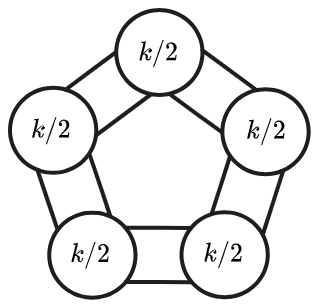
\includegraphics[scale=0.3]{5_partite_graph}
        \caption{Balanced 5-partite cycle graph on $5k/2$ vertices}
        \label{fig:5_partite_graph}
    \end{figure}
    This graph is triangle free (clear by case analysis).
    Then we see that choosing
    a vertex from each of the 5 supernodes gives a distinct 5-cycle so there are at
    least $\left(\frac{k}{2}\right)^5$ pentagons in the graph (this is actually exact). But
    $|G|=\frac{5k}{2}$ and $\Delta(G)=k$ so we can rewrite this as
    $\left(\frac{k}{2}\right)^5 = \frac{|G|}{5}\left(\frac{\Delta(G)}{2}\right)^4$ meeting
    the bound. We can do this for any even $k=\Delta(G)$ so this holds asymptotically.
\end{proof}


\section{Reductions}

First we argue that an asymptotic bound suffices. Essentially, this is true as any small
graph with a high pentagon density can be expanded to arbitrary high degree.
\begin{lemma}
    \label{lemma:pentagon_asymp_suffices}
    If $P(G) \lesssim \lambda|G|\Delta(G)^4$ as $\Delta(G)\to\infty$ for
    $G$ triangle free
    then $P(G) \leq \lambda|G|\Delta(G)^4$ for all triangle free $G$.
\end{lemma}

\begin{proof}
    More precisely our condition states that for any $\Delta$-increasing sequence of
    triangle free graphs $(G_k)_{k\in\N}$ we have
    $\limsup_{k\to\infty} \frac{P(G_k)}{|G|\Delta(G)^4} \leq \lambda$.

    Assume then for sake of contradiction that there exists $G_0$ triangle free
    such that $\frac{P(G_0)}{|G_0|\Delta(G_0)^4} > \lambda$.
    Let $\delta := \frac{P(G_0)}{|G_0|\Delta(G_0)^4}$ and consider the following
    sequence of graphs $(G_k)_{k\in\N}$: Start with $G_0$ and construct
    $G_{i+1}$ from $G_i$ by doubling every vertex of $G_i$, then for every
    $u\sim v$ in $G_i$ connect both copies of $u$ to both copies of $v$.

    \begin{figure}[!ht]
        \centering
        
\includegraphics[scale=1.5]{pentagon_asymp_construction}
    \end{figure}

    Then we have $|G_{i+1}| = 2|G_i|$ and $\Delta(G_i) = 2\Delta(G_{i+1})$ for all
    $i\in\N$. Note also that $G_i$ triangle free implies $G_{i+1}$ triangle free.
    To see this consider assume $G_i$ triangle free and $G_{i+1}$ has a triangle
    $\{u, v, w\}$. As each of $u,v,w$ are connected they must be copies of three
    different nodes from $G_i$. However such copies are connected iff their originals are
    connected so there must be a corresponding triangle in $G_i$ which is a contradiction.
    Hence each $G_i$ is triangle free.

    Take any pentagon in $G_i$. This correspond to $2^5$ pentagons in $G_{i+1}$. Each
    such pentagon in $G_{i+1}$ we get by expanding a $C_5$ in $G_i$ comes from
    some unique pentagon in $G_i$ hence $P(G_{i+1}) \geq 2^5P(G_i)$ for all $i\geq 1$.
    Hence for every $i\in\N$ we have
    \[
        \frac{P(G_i)}{|G_i|\Delta(G_i^4)} \geq
        \frac{(2^5)^i P(G_0)}{2^i|G_0|(2^i\Delta(G_0))^4}
        = \frac{2^{5i} P(G_0)}{2^{5i}|G_0|\Delta(G_0)^4}
        = \delta
    \]
    and in particular
    \[
        \limsup_{k\to\infty}\frac{P(G_k)}{|G_k|\Delta(G_k)^4} \geq
        \liminf_{k\to\infty}\frac{P(G_k)}{|G_k|\Delta(G_k)^4}
        \geq \delta > \lambda
    \]
    but $(G_k)_{k\in\N}$ is a $\Delta$-increasing sequence of triangle free graphs
    so this contradictions our assumption. Hence no such $G_0$ exists.
\end{proof}

Now we show not only is it enough to show this bound asymptotically, it also suffices
to show the bound only for regular graphs.

\begin{lemma}
    For any triangle free $G$ there exists a regular triangle free $G'$ such that
    $\Delta(G')=\Delta(G)$ and
    \[
        \frac{P(G')}{|G'|\Delta(G')^4} \geq
        \frac{P(G)}{|G|\Delta(G)^4}
    \]
\end{lemma}

\begin{proof}
    Let $G_0$ be such a triangle free graph. Construct a sequence $(G_k)_{k\in\N}$ as
    follows: To construct $G_{i+1}$ take two copies of $G_i$ then for each vertex $v\in V(G_i)$
    with $\deg v < \Delta(G_i)$ add an edge to $G_{i+1}$ between the two copies of $v$.

    \begin{figure}[!ht]
        \centering
        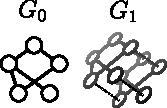
\includegraphics[scale=1.75]{wlog_regular_pentagon}
    \end{figure}

    We show by induction that each $G_i$ is triangle free, $\Delta(G_i)=\Delta(G_0)\ \forall i\in\N$
    and $\frac{P(G_i)}{|G_i|\Delta(G_i)^4} \geq \frac{P(G_0)}{|G_0|\Delta(G_0)^4}$.
    $G_0$ satisfies these conditions
    by assumption; Assume they hold for $G_i$. First we argue that $G_{i+1}$ has no
    triangles. Clearly each copy of $G_i$ has no triangles so we need to show the
    addition of edges between two 2 copies of $G_i$ doesn't induce any triangles.
    Each edge we add is between two copies of a vertex $v\in V(G_i)$. This means
    each vertex in $G_{i+1}$ has at most 1 neighbour outside of its own copy of $G_i$.
    Therefore adding an edge between two copies of some $v$ cannot induce a 3-cycle
    as the neighbourhoods of each copy of $v$ will be disjoint so $G_{i+1}$ is
    triangle free. Next we show $\Delta(G_{i+1})=\Delta(G_i)=\Delta(G_0)$; This is
    clear as we add an edge only to vertices $v$ which have $\deg v < \Delta(G_i)=\Delta(G_0)$
    meaning we do not increase the maximum degree.
    Finally we show that
    $\frac{P(G_{i+1})}{|G_{i+1}|\Delta(G_{i+1})^4} \geq \frac{P(G_0)}{|G_0|\Delta(G_0)^4}$.
    This is also easy as $|G_{i+1}|=2|G_i|$ but $P(G_{i+1}) \geq 2 P(G_i)$ as we take
    two copies of $G_i$.

    Finally we note that the minimum degree increases by 1 every iteration if the
    graph is non-regular: $\delta(G_i) < \Delta(G_i) \implies \delta(G_{i+1})=\delta(G_i) + 1$.
    Then as $\Delta(G_i)=\Delta(G_0)\forall i\in\N$ this means there can be at most
    $\Delta(G_0)-\delta(G_0) \leq \Delta(G_0)$ iterations until we arrive at a regular
    $G_k$. We found then a regular graph $G_k$ which satisfies our conditions.
\end{proof}

\begin{corollary}
    \label{corollary:pentagon_regular_suffices}
    It suffices to show that $\frac{P(G)}{|G|\Delta(G)^4} \lesssim \lambda$
    only for regular triangle free $G$.
\end{corollary}

\begin{proof}
    Assume the bound holds for regular graphs.
    Assume then for contradiction that
    there is some triangle free $\Delta$-increasing sequence $(G_k)_{k\in\N}$
    such that $\lim_{k\to\infty} \frac{P(G_k)}{|G_k|\Delta(G_k)^4} > \frac{1}{5\cdot 8}$.
    Then by the previous lemma we can construct a sequence
    $(G_k')_{k\in\N}$ where each $G_k'$ is triangle free and regular
    such that $\Delta(G_k')=\Delta(G_k)$ and
    $\frac{P(G_k')}{|G_k'|\Delta(G_k')^4} >\frac{P(G_k)}{|G_k|\Delta(G_k)^4}$
    for all $k\in\N$. Hence this is a $\Delta$-increasing triangle free regular
    sequence such that
    \[
        \limsup_{k\to\infty} \frac{P(G_k')}{|G_k'|\Delta(G_k')}
        \geq
        \lim_{k\to\infty} \frac{P(G_k)}{|G_k|\Delta(G_k)}
        > \lambda
    \]
    which is a contradiction.
\end{proof}

Now we know we only need to prove the bound asymptotically for regular graphs.
The final reduction step is the following simple lemma
\begin{lemma}
    \label{lemma:pentagon_local_count}
    Let $P(G, v)$ be the number of pentagons in $G$ containing $v$. If we have some
    $\lambda \in \R$ such that
    $\frac{P(G, v)}{\Delta(G)^4} \lesssim \lambda$ as $\Delta(G)\to\infty$
    then
    $\frac{P(G)}{|G|\Delta(G)^4} \lesssim \frac{1}{5}\lambda$ as $\Delta(G)\to\infty$.
\end{lemma}

\begin{proof}
    Note $\sum_{v\in V(G)}P(G, v) = 5P(G)$. Hence
    \begin{multline*}
        \frac{P(G)}{|G|\Delta(G)^4}
        = \frac{\sum_{v\in V(G)} P(G, v)}{5|G|\Delta(G)^4}
        = \frac{\sum_{v \in V(G)} \lambda\Delta(G)^4 + o(\Delta(G)^4)}{5|G|\Delta(G)^4}\\
        = \frac{\lambda|G|\Delta(G)^4 + o(|G|\Delta(G)^4)}{5|G|\Delta(G)^4}
        = \frac{\lambda}{5} + o(1)
    \end{multline*}
\end{proof}

Now we see how our proof of theorem \ref{thm:simple_pentagon_bound} will go.
We need only show that for a regular triangle free graphs $G$ and
$v\in V(G)$ we have an asymptotic bound of $P(G, v) \lesssim \frac{\Delta(G)^4}{8}$.
This is something that local flags can prove.

Unfortunately we know that this approach cannot be directly improved to show the
full $\frac{|G|}{5}\frac{\Delta(G)^4}{16}$ bound as this result is tight:

\begin{lemma}
    \label{lemma:pentagon_1_8_tight}
    There exists regular graphs $G$ with arbitrarily large $\Delta(G)$ such that
    some $v\in V(G)$ sits on $\frac{|G|}{5}\frac{\Delta(G)^4}{8}$ 5-cycles.
\end{lemma}

\begin{proof}
    For any $k\in\N$ even we construct the following graph: Construct a blowup of the 6-cycle
    of size $k/2$. This consists of 6 independent sets of size $k/2$ which are densely
    connected to their neighbours in a 6-cycle.
    We then add a single extra vertex which will be our distinguished vertex $v\in V(G)$ and
    connect it to densely to 2 of the supernodes which are on opposite ends of the cycle.

    \begin{figure}[!ht]
        \centering
        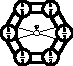
\includegraphics[scale=4]{hexagon_bound_example}
    \end{figure}

    This graph is almost regular in that every vertex has degree $k$, except those
    in the 2 supernodes connected to $v$ which have degree $k+1$. This is a detail that
    doesn't matter and could be addressed but would distract from the core of the construction.
    Asymptotically speaking this construction is regular.

    Note then that we can construct a pentagon going through $v$ by first choosing
    a vertex from each of the connected supernodes which is $\left(\frac{k}{2}\right)^2$
    choices. Then we can choose the final 2 vertices of the pentagon by either going
    "up" or "down" and picking any vertex from each of the supernodes. This gives us
    $2\left(\frac{k}{2}\right)^2$ choices leading to an overall number of
    $\frac{k^4}{8}$ 5-cycles as required.
\end{proof}

\section{Local Flags for Regular Graphs}
\label{sec:local_flags_regular_graphs}

We show now why focusing on only regular graphs is so powerful in the context of
local flags. As we saw in section \ref{sec:semidefinite_method} we want to find
interesting elements of the semantic cone $\SemCone^\emptyset$. This is dual to
finding general linear relations of density limits of local flags.

Let $\Gcl$ be a class of regular graphs.
We start by defining the extension of a flag:

\begin{definition}[Extension]
    Let $\sigma$ be a type of size $k$. Then we define the
    \textbf{extension} $\ext^\sigma_i$ as the sum of all $\sigma$ flags $\in\HeredG{}^\sigma$
    of size $k+1$ which have an edge between the unlabelled vertex the and vertex labelled $i$.
\end{definition}

\begin{note}
    By lemma \ref{lemma:local_if_connected} such flags are all local flags so
    $\ext^\sigma_i \in \Lcl^\sigma$.
\end{note}

\begin{example}
    Let $\Gcl$ be the class of red-black vertex coloured regular graphs then
    see figure \ref{fig:extension_example} for an example $\sigma$ and two possible
    extensions of $\sigma$ corresponding to extending on vertex 1 or 2.
    \begin{figure}[ht]
        \centering
        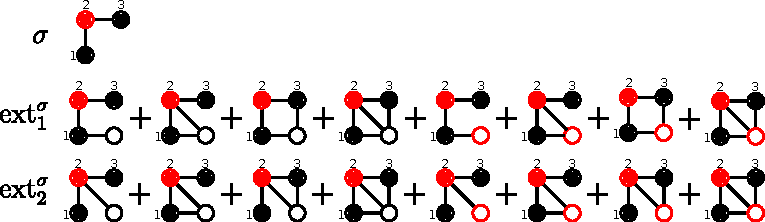
\includegraphics{extension_example}
        \caption{Example type $\sigma$ with two possible extensions}
        \label{fig:extension_example}
    \end{figure}
\end{example}

These extensions are important for the following reason:

\begin{lemma}
    If $\Gcl$ consists of only regular graphs then for any $\sigma$ and $\phi\in\Phi^\sigma$ we have
    $\phi(\ext_i^\sigma) = 1\ \forall\ i \in [|\sigma|]$.
\end{lemma}

\begin{proof}
    Let $\ext_i^\sigma=\sum_{\alpha\in I}F_\alpha$ for some index set $I$. Let
    $(G,\eta)$ be any $\sigma$-flag with $G\in\Gcl$. Then any instance of some
    $F_\alpha$ is a subset $\im\eta \subseteq U \subseteq V(G)$ where
    $G[U] \cong F_\alpha$. In particular $|U|=|F_\alpha|=|\sigma|+1=|\im\eta| + 1$ so
    $U = \im\eta \cup \{v\}$ for some $v\in V(G)$. In particular by definition of
    $\ext_i^\sigma$ this $v$ must be connected in $G$ to $\eta(i)$. Hence
    $v \in N(\eta(i))\setminus \im\eta$. This map from a copy of $F_\alpha$ in $G$ to
    a specific vertex is injective as we can
    take the $\sigma$-flag $(G[\im\eta\cup\{v\}], \eta)$ which must be isomorphic
    to $F_\alpha$. This map is also surjective for the same reason, given any
    $v\in N(\eta(i)) \setminus \im\eta$ we take $G[\im\eta \cup \{v\}$ which must
    be isomorphic to some flag $F_\alpha$ where the unlabelled vertex is connected to
    the vertex labelled $i$, so appears in the $\ext_i^\sigma$ expression.

    Therefore $\sum_{\alpha\in I}c(F_\alpha; (G,\eta)) = |N(\eta(i))\setminus\im\eta|$.
    In particular then
    \[
        \rho(\ext_i^\sigma; (G,\eta))
        = \sum_{\alpha \in I} \frac{c(F_\alpha; (G,\eta)}{\Delta(G)}
        = \frac{|N(\eta(i)) \setminus \im\eta|}{\Delta(G)}
    \]
    The size of $\im\eta$ is constant and $|N(\eta(i))|=\Delta(G)$ so this is
    in the range $[1-\frac{|\im\eta|}{\Delta(G)}, 1]$. Hence
    $\rho(\ext^\sigma_i; (G,\eta)) = 1 - o(1)$ so we do get that
    $\phi(\ext_i^\sigma)=1\ \forall\ \phi\in\Phi^\sigma$.
\end{proof}

\begin{note}
    This proof only really required that sequences of graphs in $\Gcl$ are
    \textit{asymptotically} regular so the conditions for this lemma could be relaxed
    slightly.
\end{note}

\begin{corollary}
    For any type $\sigma$ and $\phi\in\Phi^\sigma$ we
    have $\phi(\ext_i^\sigma - \ext_j^\sigma) = 0$ for all $i,j \in [|\sigma|]$
    and $\phi(f \cdot \ext_i^\sigma) = \phi(f)$ for all
    $f \in \Lcl^\sigma, i \in [|\sigma|]$.

    In particular $\ext_i^\sigma - \ext_j^\sigma$,
    $f\cdot \ext_i^\sigma - f$ and $f - f\cdot\ext_i^\sigma$ are all
    elements of the semantic cone $\SemCone^\sigma$.
\end{corollary}

\begin{corollary}
    \label{corollary:unlabel_extension}
    If $\sigma$ is a local type then for any $\phi\in\Phi^\emptyset$ we have
    $\phi(\llbracket \ext_i^\sigma - \ext_j^\sigma\rrbracket) = 0$
    for all $i,j\in [|\sigma|]$ and
    $\phi(\llbracket f \cdot \ext_i^\sigma\rrbracket) = \phi(\llbracket f \rrbracket)$
    for all $f\in\Lcl^\sigma$ and $i\in [|\sigma|]$.
\end{corollary}

\begin{proof}[Proof of Corollary \ref{corollary:unlabel_extension}]
    By the previous corollary $\ext_i^\sigma - \ext_j^\sigma$ are in the
    semantic cone $\SemCone^\sigma$ so by lemma \ref{lemma:local_pos_preserve}
    we must have $\llbracket \ext_i^\sigma - \ext_j^\sigma \rrbracket \in \SemCone^\sigma$
    so $\phi(\llbracket \ext_i^\sigma - \ext_j^\sigma\rrbracket) \geq 0$.
    The same goes for swapping $i$ and $j$ so
    $\phi(\llbracket \ext_j^\sigma - \ext_i^\sigma\rrbracket) \geq 0$
    implying $\phi(\llbracket \ext_i^\sigma - \ext_j^\sigma\rrbracket) = 0$.

    The same argument works for $\llbracket f\cdot\ext_i^\sigma \rrbracket$ and
    $\llbracket f\rrbracket$.
\end{proof}

\begin{note}
    These relations suggest that if we focused only on regular graph classes
    from the beginning we could have quotiented out the set of relations
    $\llbracket \ext_i^\sigma - \ext_j^\sigma\rrbracket$ from our vector space $\R\HeredG^\emptyset$
    to get a "cleaner" algebra. We have not verified that this is possible. If this is true
    it could theoretically enable us to generate smaller semidefinite programs but we would
    need an algorithmic way of reducing vectors over this subspace which prima facie is not
    a straightforward task.
\end{note}

The value of these results for us is twofold: Firstly, this gives us a wide set of
easy to generate elements of the semantic cone which we can use in our semidefinite
program. Secondly, this property where
$\phi(\llbracket f \rrbracket)=\phi(\llbracket f \cdot \ext_i^\sigma\rrbracket)$ gives
us a way of expressing a vector in a subspace of larger flags. In particular multiplying by
$\ext_i^\sigma$ gives a vector over flags which are 1 larger than those in the original
vector. This will be very useful to us.

\section{Counting Pentagons with Local Flags}
\label{sec:counting_pentagons}

We want to use local flags to show an asymptotic bound that for any regular, triangle free
graph $G$ we have
$P(G, v) \lesssim \frac{\Delta(G)^4}{8}$ for any $v \in V(G)$.
We first reduce this to a problem on coloured graphs.

Let $\Gcl$ be the class of red-black vertex coloured graphs which are triangle free,
regular and such that for each $G\in\Gcl$ the number of black vertices
in $G$ is exactly $\Delta(G)$ and the set of black vertices in $G$ is independent.
Note then that $\HeredG$ is the same class without the regularity as all other
properties are hereditary.

Then we have the following reduction:

\begin{lemma}
    \label{lemma:brrb_suffices}
    Let $\brrb$ be the black-red-red-black path. Then for any $\lambda\in\R$
    $\frac{c(\brrb; G)}{\Delta(G)^4} \lesssim \lambda$ as
    $\Delta(G) \to \infty$ over $\Gcl$ implies $\frac{P(H, v)}{\Delta(H)^4}\lesssim\lambda$
    as $\Delta(H)\to\infty$ over the class of regular triangle free graphs.
\end{lemma}

\begin{proof}

    Let $G$ be a simple regular triangle free graph and fix some $v\in V(G)$. Then
    $|N(v)| = \Delta(G)$ and the set $N(v)$ is independent.

    Any pentagon containing $v$ then must contain 2 vertices of $N(v)$ and 2 vertices
    outside of $N(v)$. In particular if we construct a 3-vertex-coloured graph $H$
    which is a copy of $G$ where $v$ is green, $N(v)$ is black and all others are
    red then we want to count how many pentagons contain 1 green vertex, 2 black vertices
    and 2 red vertices. Then as all black vertices are connected to the green vertex it
    suffices to count how many black-red-red-black paths there are in $H$. In fact
    removing $v$ from $H$ has no effect on this count so WLOG we can remove it.

    \begin{figure}[!ht]
        \centering
        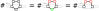
\includegraphics[scale=1.45]{pentagon_reduction}
    \end{figure}

    This $H$ graph has (up to asymptotically 0 terms) the same max degree as $G$
    so any bound on $H$ asymptotically applies to $G$.
\end{proof}

\subsection{Local Flags Setup}

We have decided on a class of graphs $\Gcl$ so we need to now find a description of
the local $\sigma$-flags.

\begin{lemma}
    \label{lemma:pentagon_local_flags}
    A $\sigma$-flag $F$ is a local $\sigma$-flag (relative to our choice of
    $\Gcl$) iff each connected component of $F$ contains a labelled vertex or a
    black vertex.
\end{lemma}

\begin{proof}
    First we show if each connected component of $F$ contains a labelled or black
    vertex then $F$ has bounded density function. We do this by induction on $|F|-|\sigma|$.
    The base case is that $|F|=|\sigma|$ which implies $F$ consists only of labelled
    vertices meaning $c(F; G) = 1 \in O(\Delta(G)^0)$ for any $G\in\Gcl^\sigma$
    as required.

    Otherwise assume $|F|>|\sigma|$. Note then that as each connected component of
    $F$ contains at least one labelled or black vertex each vertex $u$ of $F$ has a
    finite minimum distance $d(u)$ to some labelled or black vertex (where
    $d(u)=0$ for all black and labelled $u$ and $d(u) > 0$ for all unlabelled red vertices).
    Let $v$ be some unlabelled vertex in $F$ with maximum $d(v)$. Consider then removing $v$ from
    $F$: $F' := F[V(F)\setminus \{v\}]$. This $F'$ must not have any connected
    components with no black or labelled vertices because we chose $d(v)$ large as
    possible. Hence $c(F'; G) \in O\left(\Delta(G)^{|F|-|\sigma|-1}\right)$ by our
    induction hypothesis.

    Consider then some subset $\im\eta\subseteq U' \subseteq V(G)$ such that
    $G[U'] \cong F'$. We want to bound how many copies $U$ of $F$ can we obtain
    by adding one more vertex $u\in V(G)$ onto which our removed $v$ can be mapped.
    There are 2 cases: If the $v\in V(F)$ we removed was a black vertex then
    $u$ must be a black vertex, there are only $\Delta(G)$ of those meaning there
    are $\leq \Delta(G)$ possible such $U$'s. Otherwise $v$ was a red vertex
    meaning it was connected to $V(F)\setminus\{v\}$. This means $u$ must be
    in the neighbourhood of one of the vertices of $U$ of which there are
    $O(\Delta(G))$ such options. In either case there are only $O(\Delta(G))$ such
    extensions of $U'$.
    In particular though every copy $U$ of $F$ can be reached in this way. This is easily
    seen by taking any such copy and removing the vertex $u$ that $v$ is mapped to, this must
    give you a copy $U'$ of $F'$ with which we can re-add $u$ to get back to $U$.
    Therefore this process counts all copies $U$ of $F$ in $G$ giving us a bound of
    $c(F'; G) \cdot O(\Delta(G)) = O\left(\Delta(G)^{|F|-|\sigma|}\right)$ as required.

    Now that we know any such $F$ has bounded density function we simply note that
    any label extension of $F$ gives you a new flag which also has a labelled or
    black vertex in each connected component. Therefore label extension preserves
    bounded density functions so $F$ is a local $\sigma$-flag.

    We also show that this encapsulates all local $\sigma$-flags. This isn't strictly
    required for our application so I give a brief idea of the proof. Taking any
    flag with a connected component consisting of all unlabelled red vertices we can
    easily construct a sequence of graphs $(G_k)_{k\in\N}$ in $\Gcl$ where we keep
    increasing the number of copies of the unlabelled red component. We can do this maintaining
    the fact that each $G_k$ is regular and has only $\Delta(G)$ black vertices. Then
    the number of copies of $F$ increases unbounded along this sequence proving $F$ is not
    local.
\end{proof}

Now that we know our set of local flags, which tells us our local types by
lemma \ref{lemma:local_type_equiv} we can now formulate our problem as a semidefinite
problem.

\section{The Semidefinite Program}
\label{sec:pentagon_sdp}

We fixed our class of graphs $\Gcl$ to be the class of red-black vertex coloured
regular triangle-free graphs with $\Delta(G)$ black vertices such that the set of
black vertices is independent.
We want to asymptotically bound the number of black-red-red-black paths in this
class. This means we have the following objective function: $\brrb$.
This is a local flag by lemma \ref{lemma:pentagon_local_flags}. We will now use
the semidefinite method (section \ref{sec:semidefinite_method}) to find a bound
$\lambda\in\R$ such that $\phi(\brrb)\leq \lambda\ \forall\ \phi\in\Phi^\sigma$.

\begin{note}
    It proves to be more intuitive to describe our problem in terms of maximising
    $\phi(\brrb)$. We then use duality (section \ref{sec:sdp_duality}) to convert
    this to a problem of finding some $\lambda\emptyset - \brrb\in\SemCone^\emptyset$
    which proves the $\lambda$ upper bound rigorously.
\end{note}

We need to pick a subspace of $\Lcl^\emptyset$ to optimise our objective
function over. A standard method (e.g. \cite{grzesikFlagAlgebrasExtremal2014},
\cite{cummingsMonochromaticTrianglesThreecoloured2013}) is picking the subspace spanned by flags
of some fixed size. In this case it suffices to consider the subspace of flags of
size 5.\footnote{Picking larger flags intuitively allows the search to find tighter bounds but
comes at the cost of computation time}.

By our choice of subspace we need to find a vector $f$ over flags of size 5 such that
bounding $\phi(f)$ gives a bound on $\phi(\brrb)$. To achieve this we view
$\brrb$ as a $\brrb$-flag in itself: $\brrbmarked$.
Letting $\sigma=\brrb$ we note that $\sigma$ is a local type and we can compute
$\llbracket \brrbmarked \rrbracket=\frac{2}{4!}\brrb = \frac{1}{12}\brrb$.
We can then compute $\ext_1^\sigma$ and then use corollary \ref{corollary:unlabel_extension}
which tells us that
\[
    \frac{1}{12}\phi(\brrb) = \phi(\llbracket \brrbmarked \rrbracket)
    = \phi(\llbracket \brrbmarked \cdot \ext_1^\sigma\rrbracket).
    = \phi(\llbracket \ext_1^\sigma\rrbracket).
\]
where we used that $\sigma$ is the unit of the algebra $\Lcl^\sigma$. Then
$\ext_1^\sigma$ is a vector of flags of size 5: See figure \ref{fig:pentagon_objective}.
It suffices then to try to maximise $\llbracket \ext_1^\sigma\rrbracket$: Call this
vector $O$.

\begin{figure}[ht]
    \centering
    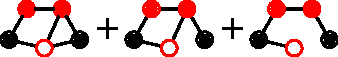
\includegraphics{pentagon_objective}
    \caption{$\ext^\sigma_1$ where $\sigma=\brrb$}
    \label{fig:pentagon_objective}
\end{figure}

To apply our semidefinite method we first need a list of known elements of the
semantic cone $\SemCone^\emptyset$ or dually a list of linear constraints on limit functionals.
For any type $\sigma$ we immediately get the elements
$\llbracket \ext^\sigma_i - \ext_j^\sigma\rrbracket$ from corollary
\ref{corollary:unlabel_extension}. We want only those that are in the subspace of
flags of size 5 so we take all such vectors where $|\sigma|=4$.

We know that in any $G\in\Gcl$ the set of black vertices is independent and has size
$\Delta(G)$. Let $B_k$ be the $\emptyset$-flag consisting of $k$ independent black
vertices. e.g. $B_1=\vertex, B_2=\nonedge, B_3=\triangleempty,\dots$. Then we know $c(B_k; G) = \binom{\Delta(G)}{k}$
for any $G\in\Gcl$ which implies $\phi(B_k)=1\ \forall\ \phi\in\Phi^\emptyset\ \forall\ k\in\N$.
We would like to add these to the list of constraints. For $k=5$ this is already in
the subspace of flags of size 5 so we can add it directly. For $k < 5$ we need
to do the same extension trick as with our objective function where we use that
$\llbracket B_k \rrbracket = B_k$ to get
\begin{multline*}
    1 = \phi(B_k)=\phi(\llbracket B_k \rrbracket)
    = \phi(\llbracket B_k \cdot \ext_1^{B_k}\rrbracket)
    = \phi\left(\left\llbracket B_k \cdot \left(\ext_1^{B_k}\right)^{5-k}\right\rrbracket\right)\\
    = \phi\left(\left\llbracket \left(\ext_1^{B_k}\right)^{5-k}\right\rrbracket\right).
\end{multline*}
$\left(\ext_1^{B_k}\right)^{5-k}$ is a vector over flags of size 5 so this is
a constraint we can use.

Finally then we want to encode constraints of the form $\phi(\llbracket f^2 \rrbracket) \geq 0$
for all $f\in \Lcl^\sigma$. To do this we need to find local types $\sigma$ and sizes $n$
such that $f^2$ is an expression of flags of size 5 for all $f\in\Glocn^\sigma$.
Those pairs $(\sigma, n)$ are ($\vertex$, $3$), ($\triangleempty$, $4$), ($\pentsqtypeone$, $4$),
($\pentsqtypetwo$, $4$), ($\pentsqtypethree$, $4$), and ($\pentsqtypefour$, $4$).

Let $\Bcl=(F_1, \dots, F_\ell)$ be the basis of all flags of size 5.
In summary then our problem is:
\begin{align*}
    \max_{x\in\R^\ell}\ \ &\ \phi_x(O)\\
    \text{such that}\ \ &\ \phi_x(F_i) \geq 0\ \forall\ i \in [\ell]\\
    &\ \phi_x(\llbracket \ext^\sigma_i - \ext^\sigma_j\rrbracket) = 0\ \forall\
    |\sigma|=4, i, j \in [4]\\
    &\ \phi_x(B_5) = 1\\
    &\ \phi_x\left(\left\llbracket\left(\ext_1^{B_k}\right)^{5-k}\right\rrbracket\right) = 1\
    \forall\ k \in [4]\\
    &\ \phi_x(\llbracket f^2 \rrbracket) \geq 0 \forall f \in \Lcl_n^\sigma\ \forall (\sigma, n)
    \ \text{from above list}.
\end{align*}

We know from section \ref{sec:semidefinite_method} how to construct the corresponding
SDP. A solution to this SDP finds a convex combination of elements of the semantic cone
which prove an upper bound on $\phi(O)\ \forall\ \phi\ \in \Phi^\emptyset$.

We use a SDP solver (see appendix \ref{app:flag_software}) to show the following result:
\begin{lemma}
    \label{lemma:pentagon_1_4_bound}
    \[
        \frac{1}{4}\emptyset - O \in \SemCone^\emptyset.
    \]
\end{lemma}
In the next section (\ref{sec:pentagon_proof_validation}) we will show how we make this
SDP solution rigorous. For now we show that this bound suffices to prove theorem
\ref{thm:simple_pentagon_bound}.

\begin{proof}[Proof of theorem \ref{thm:simple_pentagon_bound}]
    By lemma \ref{lemma:pentagon_1_4_bound} we have that
    $\phi(O) \leq \frac{1}{4}\ \forall\ \phi\in\Phi^\sigma$.
    We know that $\frac{1}{12}\phi(\brrb)=\phi(O)$ so $\phi(\brrb) \leq 3$.
    Therefore for any $\Delta$-increasing sequence of graphs $(G_k)_{k\in\N}$ we have
    $\lim_{k\to\infty} \frac{c(\brrb; G_k)}{\binom{\Delta(G_k)}{4}} \leq 3$.
    Intuitively then $\binom{\Delta(G_k)}{4}$ is asymptotically $\frac{\Delta(G_k)^4}{4!}$ so
    we get $\lim_{k\to\infty} c(\brrb; G_k) \leq \frac{3}{4!} = \frac{1}{8}$.
    We show this argument more precisely now:

    We use the fact that
    $\frac{\Delta(G_k)!}{(\Delta(G_k)-4)!} = \Delta(G_k)^4 + o(\Delta(G_k)^4)$
    to show that
    \[
        \begin{split}
            \lim_{k\to\infty}\frac{c(\brrb; G_k)}{\Delta(G_k)^4}
            &= \lim_{k\to\infty}\frac{c(\brrb; G_k)}{\binom{\Delta(G_k)}{4}}
            \frac{\Delta(G_k)!}{4!(\Delta(G_k)-4)!\Delta(G_k)^4}\\
            &= \lim_{k\to\infty}\frac{c(\brrb; G_k)}{\binom{\Delta(G_k)}{4}}
            \frac{\Delta(G_k)^4 + o(\Delta(G_k)^4}{4!\Delta(G_k)^4}\\
            &= \lim_{k\to\infty}(1+o(1))\frac{1}{4!}\frac{c(\brrb; G_k)}{\binom{\Delta(G_k)}{4}}\\
            &\leq \frac{1}{8}.
        \end{split}
    \]
    Then by lemma \ref{lemma:brrb_suffices}
    $\frac{P(G, v)}{\Delta(G)^4}\lesssim \frac{1}{8}$ for any regular triangle free
    $G$ and $v \in V(G)$.
    Lemma \ref{lemma:pentagon_local_count} tells us then
    $\frac{P(G)}{|G|\Delta(G)^4}\lesssim \frac{1}{5\cdot 8}$ for any regular triangle
    free $G$. Corollary \ref{corollary:pentagon_regular_suffices} shows that
    we can drop the regular requirement.
    Finally, lemma \ref{lemma:pentagon_asymp_suffices} shows that this
    asymptotic bound implies the non-asymptotic bound.
    \[
        \therefore P(G) \leq \frac{|G|}{5}\frac{\Delta(G)^4}{8}
        \ \forall\ G\ \text{triangle free}.
    \]
\end{proof}

\section{SDP Proof Validation}
\label{sec:pentagon_proof_validation}

We've shown in the previous section how to express our problem in the form of a
semidefinite program and we claimed that SDP software found a solution proving a bound
of $1/8$. Clearly though appealing to a software implementation, no matter how well tested,
is not rigorous: We should verify the outcome ourselves. We saw in section \ref{sec:semidefinite_method} how such an SDP
solution corresponds to constructing a specific element of the semantic cone by taking
convex combinations of known elements of the cone. In this section we will show the
combination of elements that was found by the SDP software, verifying that it is indeed
a valid proof.

We will defer the specific details of how we converted the SDP solution into the following
proof to appendix \ref{app:sdp_verification}.

First, as a reminder we were trying to bound $\phi(O)=\frac{1}{12}\phi(\brrb)$
where we defined $O$ as an extension of $\sigma_O = \brrb$:
$O = \llbracket \ext_1^{\sigma_O}\rrbracket.$ We expand this and find that
\[
    O = \frac{1}{60}\pentF{9} + \frac{1}{120}\pentF{37} + \frac{1}{60}\pentF{55}
\]
For convenience we scale this by 120 to get
$2\pentF{9} + \pentF{37} + 2\pentF{55}$. Then we prove that
$120\phi(O) \leq\lambda\ \forall\ \phi\in\Phi^\emptyset$ by showing
$\lambda\emptyset - 2\pentF{9} + \pentF{37} + 2\pentF{55}\in\SemCone^\emptyset$.

First we take $B_1=\vertex$ as defined above. We know
$1=\phi(\vertex)=\phi(\llbracket (\ext^\vertex_1)^4 \rrbracket) = \frac{1}{5}\phi(\pentF{6})$
for all $\phi\in\Phi^\emptyset$ hence 
\begin{equation}
    5\emptyset - \pentF{6} \in\SemCone^\emptyset.
    \label{eq:pent_b1}
\end{equation}

Next, by corollary \ref{corollary:unlabel_extension} for any local type $\sigma$
and $i,j \in [|\sigma|]$ and we have
$\llbracket \ext_i^\sigma - \ext_j^\sigma\rrbracket\in\SemCone^\emptyset$. It also
proves easier to scale these by $120$ as with $O$.
We compute some such vectors for the following fixed types:
$\sigma_1 := \pentsig{1}, \sigma_2 := \pentsig{2}$,
$\sigma_3 := \pentsig{3}$, $\sigma_4 := \pentsig{4}$
and $\sigma_5 := \pentsig{5}$.
\begin{align}
    120\llbracket \ext_2^{\sigma_1} - \ext_1^{\sigma_1} \rrbracket
    &=-4\pentF{4} - 6\pentF{5} + 2\pentF{12} + 2\pentF{24} + 4\pentF{32}
    \in\SemCone^\emptyset.\label{eq:pent_sig_1}\\
    120\llbracket \ext_1^{\sigma_2} - \ext_2^{\sigma_2} \rrbracket
    &= 
    24\pentF{6} - 4\pentF{13} - 4\pentF{15} - 2\pentF{18} - 2\pentF{25} - 12\pentF{33} - 6\pentF{34}
    \in \SemCone^\emptyset.\label{eq:pent_sig_2}\\
    120\llbracket \ext_2^{\sigma_3} - \ext_1^{\sigma_3} \rrbracket
    &=2\pentF{11} + \pentF{12} - 2\pentF{15} + \pentF{22} + 2\pentF{24} - 2\pentF{25}
    \label{eq:pent_sig_3}.\\
    120\llbracket \ext_2^{\sigma_4} - \ext_1^{\sigma_4} \rrbracket
    &= \pentF{8} + \pentF{12} - 2\pentF{15} + 4\pentF{31} + 4\pentF{32} - 6\pentF{34}
    \label{eq:pent_sig_4}.\\
    120\llbracket \ext_3^{\sigma_5} - \ext_1^{\sigma_5} \rrbracket
    &= -2\pentF{16} - \pentF{17} + \pentF{37} + 2\pentF{55}
    \label{eq:pent_sig_5}.
\end{align}

Now we can take a convex combination of these elements of the semantic cone to
get another element of the semantic cone.
\begin{multline}
    6\cdot (\ref{eq:pent_b1})
    + 1\cdot (\ref{eq:pent_sig_1})
    + \frac{1}{4} \cdot (\ref{eq:pent_sig_2})
    + 1\cdot (\ref{eq:pent_sig_3})
    + 1\cdot (\ref{eq:pent_sig_4})
    + 2\cdot (\ref{eq:pent_sig_5})\\
    =
    30\emptyset -4\pentF{4} - 6\pentF{5} + \pentF{8} + 2\pentF{11} + 4\pentF{12} - \pentF{13} -
        5\pentF{15} - 4\pentF{16} - 2\pentF{17} - \frac{1}{2}\pentF{18}\\
        + \pentF{22} + 4\pentF{24} - \frac{5}{2}\pentF{25} + 4\pentF{31} + 8\pentF{32} - 3\pentF{33}
        - \frac{15}{2}\pentF{34} + 2\pentF{37} + 4\pentF{55}.
    \label{eq:pent_lin_sum}
\end{multline}

Consider then the type $\sigma_6=\pentsig{6}$ and the following
vectors $f,g \in \Lcl^{\sigma_6}$.
\[
    f = -\pentcf{0}{3} + \frac{1}{4}\pentcf{0}{4} + \frac{1}{4}\pentcf{0}{5}+\frac{1}{2}\pentcf{0}{6}
    \ \ \ \ g = -\frac{1}{4}\pentcf{0}{4} + \frac{1}{4}\pentcf{0}{5}
\]
Then by \ref{lemma:local_pos_preserve} both of the following are elements of the
semantic cone:
\[
    \begin{split}
        120 \llbracket f^2 \rrbracket &= 
    4\pentF{4} - \pentF{8} - 2\pentF{11} + \pentF{13} + \frac{1}{4}\pentF{18} - \pentF{22} -
        4\pentF{31} + 3\pentF{33} + \frac{1}{4}\pentF{40} + \frac{1}{4}5\pentF{55}\\
        120 \llbracket g^2 \rrbracket &= 
        \frac{1}{4}\pentF{18} - \frac{1}{4}\pentF{40} - \frac{1}{4}\pentF{55}
    \end{split}
\]
The sum of these two elements gives a new element of the semantic cone
\begin{equation}
    4\pentF{4} - \pentF{8} - 2\pentF{11} + \pentF{13} + \frac{1}{2}\pentF{18} - \pentF{22} -
    4\pentF{31} + 3\pentF{33} \in \SemCone^\emptyset
    \label{eq:pent_cs_0}
\end{equation}

We do the same thing with the type $\sigma_7 := \pentsig{7}$: Take the following
vectors $h, \ell \in \Lcl^{\sigma_7}$.
\[
    h = -\frac{1}{2}\pentcf{1}{4} - \pentcf{1}{5} + \frac{1}{2}\pentcf{1}{7}
    \ \ \ \ \ell = \pentcf{1}{3} - \pentcf{1}{4} + \pentcf{1}{5} - \pentcf{1}{7}
\]
Then we can compute
\[
    \begin{split}
        120 \llbracket h^2 \rrbracket &= 
        -2\pentF{9} + \pentF{15} + 2\pentF{16} + \frac{1}{2}\pentF{25} + \frac{3}{2}\pentF{34} -
        \pentF{37} - 2\pentF{55}\\
        120 \llbracket g^2 \rrbracket &= 
        6\pentF{5} - 4\pentF{12} + 4\pentF{15} + 2\pentF{16} + 2\pentF{17} - 4\pentF{24} + 2\pentF{25} - 8\pentF{32}\\
        &\ \ \ + 6\pentF{34} - 2\pentF{37} - 4\pentF{55}.
    \end{split}
\]
The sum of these two elements of the semantic cone is:
\begin{multline}
    6\pentF{5} - 2\pentF{9} - 4\pentF{12} + 5\pentF{15} + 4\pentF{16} + 2\pentF{17} - 4\pentF{24} + \frac{5}{2}\pentF{25} - 8\pentF{32}\\
    + \frac{15}{2}\pentF{34} - 3\pentF{37} - 6\pentF{55}
    \in\SemCone^\emptyset
    \label{eq:pent_cs_1}
\end{multline}

Finally, we take the combination of equations \ref{eq:pent_lin_sum}, \ref{eq:pent_cs_0}
and \ref{eq:pent_cs_1} to get our final element of the cone.
\[
    (\ref{eq:pent_lin_sum}) + (\ref{eq:pent_cs_0}) + (\ref{eq:pent_cs_1})
    = 30\emptyset -2\pentF{9} - \pentF{37} - 2\pentF{55}
    \in\SemCone^\emptyset
\]
We know $120O = 2\pentF{9} + \pentF{37} + 2\pentF{55}$ so
$30\emptyset - 120O \in \SemCone^\emptyset$. This implies
$\frac{1}{4}\emptyset - O \in \SemCone^\emptyset$ as required.
This proves lemma \ref{lemma:pentagon_1_4_bound} completing our proof
of theorem \ref{thm:simple_pentagon_bound}.

\section{Proving the Stronger Result}
\label{sec:pentagon_stronger}

We can use local flags in a more complex way to get the stronger result
of theorem \ref{thm:full_pentagon_bound}.

To prove the bound in theorem \ref{thm:simple_pentagon_bound} we defined
$P(G,v)$ to be the number of pentagons containing a $v \in G$
and used local flags find an upper bound.
To prove the strong result in theorem \ref{thm:full_pentagon_bound}
we will bound the following function. For fixed $v\in G$ define
\[
    Q(G, v) := \Delta(G)P(G, v) 
    + \sum_{u \in N(v)}P(G, u).
\]

Then we claim
\begin{lemma}
    \label{lemma:pent_q_v}
    For $G$ triangle free and $v\in V(G)$
    \[
        Q(G, v) \lesssim 0.2073 \Delta(G)^5
        \ \text{as}\ \Delta(G) \to\infty
    \]
\end{lemma}

We will prove this lemma now using local flags.
We use the same class of graphs $\Gcl$ as before, where the black vertices represent
those in the neighbourhood of $v$ and the others are red.
We've seen already then how to convert a triangle free regular graph $G$ into
the corresponding $G' \in \Gcl$ such that $\rho(\brrb, G') = P(G,v)/\binom{\Delta(G)}{4}$.

Note that any pentagon passing through the neighbourhood of $v$ contains at most 2
such vertices. Therefore
\[
    \rho(\pentF{56} + 2\pentF{55}; G')
    = \frac{\sum_{u \in N(V)} P(G, v)}{\binom{\Delta(G)}{5}}.
\]
Now we use the same extensions trick from before to embed our desired vector
into a space of flags of size $n$ and get the following objective vector
\[
    O := \llbracket \brrbmarked \cdot (\ext^{\sigma_1}_1)^{n-4} \rrbracket
    + \llbracket \pentF{56marked} \cdot (\ext^{\sigma_2}_1)^{n-5} \rrbracket
    + 2\llbracket \pentF{55marked} \cdot (\ext^{\sigma_3}_1)^{n-5} \rrbracket
\]
where $\sigma_1=\brrb, \sigma_2=\pentF{56}, \sigma_3=\pentF{55}$.
Then using the exact same set of constraints as from section 
\ref{sec:pentagon_sdp} we can use an SDP solver (see appendix \ref{app:flag_software})
using flags of size $n=8$ to find:
\begin{lemma}
    \label{lemma:pentagon_stronger_bound}
    \[
        0.4146\emptyset - O \in \SemCone^\emptyset
    \]
    hence $\phi(O) \leq 0.4146\ \forall\ \phi\in\Phi^\emptyset$.
\end{lemma}
Calculating the normalising factors (definition \ref{def:averaging_normalisation})
we find this implies
\[
    \frac{2}{4!}\phi(\brrb) + \frac{2}{5!}\phi(\pentF{56} + 2\pentF{55}) \leq 0.4146
\]
Hence for any convergent $\Delta$-increasing sequence of graphs $(G_k)_{k\in\N}$
we have
\[
    \begin{split}
        \lim_{k\to\infty}\frac{2}{4!}\rho(\brrb; G_k)
        + \frac{2}{5!}\rho(\pentF{56}; G_k) + \frac{4}{5!}\rho(\pentF{55}; G_k)
        \leq 0.4146\\
        \implies
        \lim_{k\to\infty}\frac{2}{4!}\frac{c(\brrb; G_k)}{\binom{\Delta(G_k)}{4}}
        + \frac{2}{5!}\frac{c(\pentF{56}; G_k)}{\binom{\Delta(G_k)}{5}}
        + \frac{4}{5!}\frac{c(\pentF{55}; G_k)}{\binom{\Delta(G_k)}{5}}
        \leq 0.4146\\
        \implies
        \lim_{k\to\infty}2\frac{c(\brrb; G_k)}{\Delta(G_k)^4}
        + 2\frac{c(\pentF{56}; G_k)}{\Delta(G_k)^5}
        + 4\frac{c(\pentF{55}; G_k)}{\Delta(G_k)^5}
        \leq 0.4146\\
        \implies
        \lim_{k\to\infty} \frac{c(\brrb; G_k)}{\Delta(G_k)^4}
        + \frac{c(\pentF{56}; G_k)}{\Delta(G_k)^5}
        + 2\frac{c(\pentF{55}; G_k)}{\Delta(G_k)^5}
        \leq 0.2073
    \end{split}
\]
Therefore
\[
    \Delta(G)c(\brrb; G)
    + c(\pentF{56}; G)
    + 2c(\pentF{55}; G)
    \lesssim 0.2073\Delta(G)^5
\]
By construction though this proves the same bound holds for the $Q(G,v)$ function
\[
    \Delta(G)P(G, v)
    + \sum_{u \in N(V)}P(G, u)
    \lesssim 0.2073\Delta(G)^5
    \implies
    Q(G, v) \lesssim 0.2073\Delta(G)^5
\]
proving lemma \ref{lemma:pent_q_v}.

Now we can prove the full result of theorem \ref{thm:full_pentagon_bound}.
\begin{proof}[Proof of \ref{thm:full_pentagon_bound}]
    For a triangle-free regular graph $G$ we sum $Q(G, v)$ over all $v \in V(G)$:
    \[
        \begin{split}
        \sum_{v \in V(G)} Q(G,v)
            &= \sum_{v \in V(G)} \Delta(G)P(G, v) + \sum_{u \in N(V)}P(G, u)\\
            &= 5\Delta(G)P(G) + \sum_{v\in V(G)}\sum_{u \in N(V)}P(G, u)
        \end{split}
    \]
    Then as $G$ is regular we this comes out to
    \[
        \begin{split}
            \sum_{v \in V(G)} Q(G,v)
            &= 5\Delta(G)P(G) + \Delta(G)\sum_{u\in V(G)}P(G, u)\\
            &= 5\Delta(G)P(G) + 5\Delta(G)P(G)\\
            &= 10\Delta(G)P(G)
        \end{split}
    \]
    Therefore
    \[
        10\Delta(G)P(G) \lesssim 0.2073|G|\Delta(G)^5
        \implies P(G) \lesssim 0.02073|G|\Delta(G)^4
    \]
\end{proof}


\chapter*{Popular summary}
\addcontentsline{toc}{chapter}{Popular summary}
Popular summary (half to one page, in English or Dutch, accessible to a first year bachelor student in mathematics)

\printbibliography{}

\end{document}
